\documentclass[twoside]{book}

% Packages required by doxygen
\usepackage{calc}
\usepackage{doxygen}
\usepackage{graphicx}
\usepackage[utf8]{inputenc}
\usepackage{makeidx}
\usepackage{multicol}
\usepackage{multirow}
\usepackage{textcomp}
\usepackage[table]{xcolor}

% Font selection
\usepackage[T1]{fontenc}
\usepackage{mathptmx}
\usepackage[scaled=.90]{helvet}
\usepackage{courier}
\usepackage{amssymb}
\usepackage{sectsty}
\renewcommand{\familydefault}{\sfdefault}
\allsectionsfont{%
  \fontseries{bc}\selectfont%
  \color{darkgray}%
}
\renewcommand{\DoxyLabelFont}{%
  \fontseries{bc}\selectfont%
  \color{darkgray}%
}

% Page & text layout
\usepackage{geometry}
\geometry{%
  a4paper,%
  top=2.5cm,%
  bottom=2.5cm,%
  left=2.5cm,%
  right=2.5cm%
}
\tolerance=750
\hfuzz=15pt
\hbadness=750
\setlength{\emergencystretch}{15pt}
\setlength{\parindent}{0cm}
\setlength{\parskip}{0.2cm}
\makeatletter
\renewcommand{\paragraph}{%
  \@startsection{paragraph}{4}{0ex}{-1.0ex}{1.0ex}{%
    \normalfont\normalsize\bfseries\SS@parafont%
  }%
}
\renewcommand{\subparagraph}{%
  \@startsection{subparagraph}{5}{0ex}{-1.0ex}{1.0ex}{%
    \normalfont\normalsize\bfseries\SS@subparafont%
  }%
}
\makeatother

% Headers & footers
\usepackage{fancyhdr}
\pagestyle{fancyplain}
\fancyhead[LE]{\fancyplain{}{\bfseries\thepage}}
\fancyhead[CE]{\fancyplain{}{}}
\fancyhead[RE]{\fancyplain{}{\bfseries\leftmark}}
\fancyhead[LO]{\fancyplain{}{\bfseries\rightmark}}
\fancyhead[CO]{\fancyplain{}{}}
\fancyhead[RO]{\fancyplain{}{\bfseries\thepage}}
\fancyfoot[LE]{\fancyplain{}{}}
\fancyfoot[CE]{\fancyplain{}{}}
\fancyfoot[RE]{\fancyplain{}{\bfseries\scriptsize Generated on Wed Nov 22 2023 15\-:25\-:03 for R\-E\-C\-O\-S\-I\-P\-M by Doxygen }}
\fancyfoot[LO]{\fancyplain{}{\bfseries\scriptsize Generated on Wed Nov 22 2023 15\-:25\-:03 for R\-E\-C\-O\-S\-I\-P\-M by Doxygen }}
\fancyfoot[CO]{\fancyplain{}{}}
\fancyfoot[RO]{\fancyplain{}{}}
\renewcommand{\footrulewidth}{0.4pt}
\renewcommand{\chaptermark}[1]{%
  \markboth{#1}{}%
}
\renewcommand{\sectionmark}[1]{%
  \markright{\thesection\ #1}%
}

% Indices & bibliography
\usepackage{natbib}
\usepackage[titles]{tocloft}
\setcounter{tocdepth}{3}
\setcounter{secnumdepth}{5}
\makeindex

% Custom commands
\newcommand{\clearemptydoublepage}{%
  \newpage{\pagestyle{empty}\cleardoublepage}%
}


%===== C O N T E N T S =====

\begin{document}

% Titlepage & ToC
\pagenumbering{roman}
\begin{titlepage}
\vspace*{7cm}
\begin{center}%
{\Large R\-E\-C\-O\-S\-I\-P\-M \\[1ex]\large 6.\-9.\-0 }\\
\vspace*{1cm}
{\large Generated by Doxygen 1.8.5}\\
\vspace*{0.5cm}
{\small Wed Nov 22 2023 15:25:03}\\
\end{center}
\end{titlepage}
\clearemptydoublepage
\tableofcontents
\clearemptydoublepage
\pagenumbering{arabic}

%--- Begin generated contents ---
\chapter{Hierarchical Index}
\section{Class Hierarchy}
This inheritance list is sorted roughly, but not completely, alphabetically\-:\begin{DoxyCompactList}
\item I\-Conditions\-Change\-Listener\begin{DoxyCompactList}
\item \contentsline{section}{C\-A\-L\-I\-C\-E\-:\-:multi\-Calibrator}{\pageref{classCALICE_1_1multiCalibrator}}{}
\end{DoxyCompactList}
\item Processor\begin{DoxyCompactList}
\item \contentsline{section}{C\-A\-L\-I\-C\-E\-:\-:multi\-Calibrator}{\pageref{classCALICE_1_1multiCalibrator}}{}
\end{DoxyCompactList}
\item T\-Object\begin{DoxyCompactList}
\item \contentsline{section}{T\-Convolution}{\pageref{classTConvolution}}{}
\end{DoxyCompactList}
\end{DoxyCompactList}

\chapter{Data Structure Index}
\section{Class List}
Here are the classes, structs, unions and interfaces with brief descriptions\-:\begin{DoxyCompactList}
\item\contentsline{section}{{\bf C\-A\-L\-I\-C\-E\-::multi\-Calibrator} \\*Processor to add P\-A\-R\-\_\-\-M\-U\-L\-T\-I to the event and calibrate the threshold }{\pageref{classCALICE_1_1multiCalibrator}}{}
\item\contentsline{section}{{\bf T\-Convolution} \\*R\-O\-O\-T class which generates the convolution of two functions }{\pageref{classTConvolution}}{}
\end{DoxyCompactList}

\chapter{Data Structure Documentation}
\section{C\-A\-L\-I\-C\-E\-:\-:Ahc2\-Calibrate\-Processor Class Reference}
\label{classCALICE_1_1Ahc2CalibrateProcessor}\index{C\-A\-L\-I\-C\-E\-::\-Ahc2\-Calibrate\-Processor@{C\-A\-L\-I\-C\-E\-::\-Ahc2\-Calibrate\-Processor}}


Processor that does the Si\-P\-M calibration.  




{\ttfamily \#include $<$Ahc2\-Calibrate\-Processor.\-hh$>$}

Inheritance diagram for C\-A\-L\-I\-C\-E\-:\-:Ahc2\-Calibrate\-Processor\-:\begin{figure}[H]
\begin{center}
\leavevmode
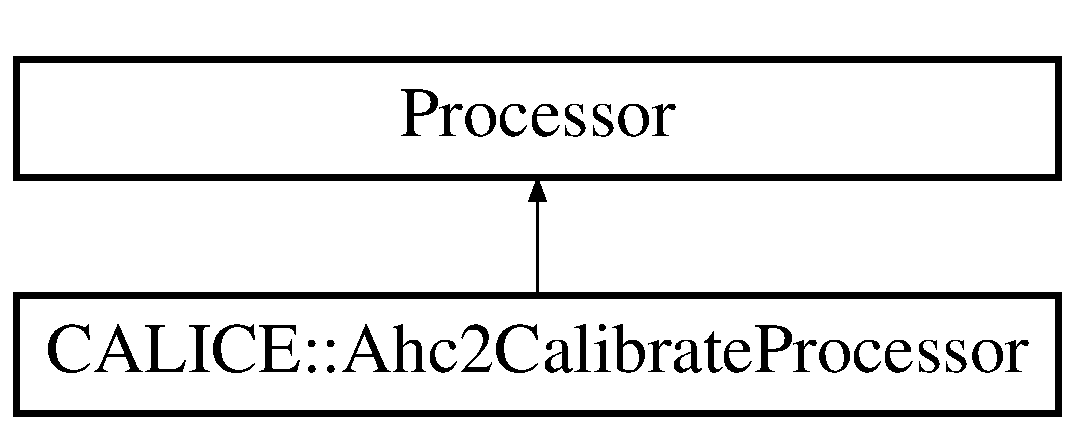
\includegraphics[height=2.000000cm]{classCALICE_1_1Ahc2CalibrateProcessor}
\end{center}
\end{figure}
\subsection*{Public Member Functions}
\begin{DoxyCompactItemize}
\item 
{\bf Ahc2\-Calibrate\-Processor} $\ast$ {\bfseries new\-Processor} ()\label{classCALICE_1_1Ahc2CalibrateProcessor_a57d619e6f0986ae6a02cbced83acc6f5}

\item 
virtual void {\bfseries init} ()\label{classCALICE_1_1Ahc2CalibrateProcessor_ad821f0bc1b0bd316e93eba7a24b7a723}

\item 
virtual void {\bfseries process\-Run\-Header} (L\-C\-Run\-Header $\ast$run)\label{classCALICE_1_1Ahc2CalibrateProcessor_ab1633c8a20a474042b7e2925276921c3}

\item 
virtual void {\bfseries process\-Event} (L\-C\-Event $\ast$evt)\label{classCALICE_1_1Ahc2CalibrateProcessor_a95d7418cc0c13b2e941f64bc222fb8b6}

\item 
virtual void {\bfseries check} (L\-C\-Event $\ast$evt)\label{classCALICE_1_1Ahc2CalibrateProcessor_a95b2468cd5bfb6ef37e3f4b4c08c2c68}

\item 
virtual void {\bfseries end} ()\label{classCALICE_1_1Ahc2CalibrateProcessor_a74e9e535f35082ecc9d311ce036324c4}

\end{DoxyCompactItemize}
\subsection*{Protected Member Functions}
\begin{DoxyCompactItemize}
\item 
void {\bfseries Fill\-Container} (L\-C\-Event $\ast$evt)\label{classCALICE_1_1Ahc2CalibrateProcessor_acaa509d1340c3afffb7f3eea852397f5}

\item 
void {\bf calibrate\-Energy\-And\-Fill\-Output\-Collections} (Ahc2\-Calibrations $\ast$calibration, const int Gain\-Bit, const int Hit\-Bit, const float raw\-Energy, const float raw\-T\-D\-C, const float time\-Reference, const int B\-X\-I\-D, const int Mem, L\-C\-Collection $\ast$ahc\-Hit\-Output\-Col, boost\-::optional$<$ std\-::pair$<$ int, int $>$ $>$ asic\-Stop\-Info)
\begin{DoxyCompactList}\small\item\em Calibrate the energy (convert from energy in A\-D\-C counts to energy in M\-I\-Ps) \end{DoxyCompactList}\item 
void {\bfseries Correct\-Occupancy} (Decoder\-Set $\ast$decoder, L\-C\-Collection $\ast$ahc\-Hit\-Output\-Col, int bxid)\label{classCALICE_1_1Ahc2CalibrateProcessor_a710d5725af93224c9e277df6994535ab}

\item 
bool {\bfseries check\-Hit} (Calorimeter\-Hit\-Impl $\ast$hit)\label{classCALICE_1_1Ahc2CalibrateProcessor_aaa5a4d84225a0455058ec8ab24f650b1}

\end{DoxyCompactItemize}
\subsection*{Protected Attributes}
\begin{DoxyCompactItemize}
\item 
std\-::string {\bf \-\_\-input\-Col\-Name}\label{classCALICE_1_1Ahc2CalibrateProcessor_af40da80c07919fd7ff11c2eea1aeb381}

\begin{DoxyCompactList}\small\item\em name of the input collection \end{DoxyCompactList}\item 
std\-::string {\bf \-\_\-input\-Col\-Name\-A\-S\-I\-C}\label{classCALICE_1_1Ahc2CalibrateProcessor_aa80531c67c2722ad0e2460a7e0876bae}

\begin{DoxyCompactList}\small\item\em Input L\-C\-I\-O Collection containig information on the stopping B\-X\-I\-S and asic of the R\-O\-C. \end{DoxyCompactList}\item 
std\-::string {\bf \-\_\-ahc\-Hit\-Output\-Col\-Name}\label{classCALICE_1_1Ahc2CalibrateProcessor_a3dc06786436feb1670498da3fd69ad94}

\begin{DoxyCompactList}\small\item\em name of the output A\-H\-C hit collection \end{DoxyCompactList}\item 
std\-::string {\bf \-\_\-mapping\-Processor\-Name}\label{classCALICE_1_1Ahc2CalibrateProcessor_ac8d1b19a0ffa72a6ea1427664503921d}

\begin{DoxyCompactList}\small\item\em name of the processor which provides the mapping \end{DoxyCompactList}\item 
std\-::string {\bf \-\_\-calib\-Processor\-Name}\label{classCALICE_1_1Ahc2CalibrateProcessor_ae410aaaebdd65ba4054169c41266154e}

\begin{DoxyCompactList}\small\item\em name of the processor which provides the Si\-P\-M calibrations \end{DoxyCompactList}\item 
std\-::string {\bfseries \-\_\-\-Ahc2\-Hardware\-Connection\-Name}\label{classCALICE_1_1Ahc2CalibrateProcessor_a58a404a600c53c93f2a8d93cdd3d0bdd}

\item 
std\-::string {\bf \-\_\-temperature\-Processor\-Name}\label{classCALICE_1_1Ahc2CalibrateProcessor_acb920d14fbddb7869a6563c9b8e0591d}

\begin{DoxyCompactList}\small\item\em name of the processor which provides the Si\-P\-M temperature \end{DoxyCompactList}\item 
std\-::string {\bf \-\_\-\-B\-I\-F\-Collection\-Name}\label{classCALICE_1_1Ahc2CalibrateProcessor_a506a8b03d3d6114e8c9372319748e9a3}

\begin{DoxyCompactList}\small\item\em name of the input collection \end{DoxyCompactList}\item 
std\-::string {\bf \-\_\-cell\-Description\-Processor\-Name}\label{classCALICE_1_1Ahc2CalibrateProcessor_abb12c048f5ca0a876f4112580dcd790e}

\begin{DoxyCompactList}\small\item\em name of the processor which provides the cells description \end{DoxyCompactList}\item 
Mapped\-Container\\*
$<$ Cell\-Description $>$ $\ast$ {\bf \-\_\-cell\-Descriptions}\label{classCALICE_1_1Ahc2CalibrateProcessor_a9569a1acebd769a434928d339a069eb3}

\begin{DoxyCompactList}\small\item\em mapped container of cells description \end{DoxyCompactList}\item 
bool {\bf \-\_\-scale\-Energy}\label{classCALICE_1_1Ahc2CalibrateProcessor_aef2b11d192204ebb3723fb47fe6a0976}

\begin{DoxyCompactList}\small\item\em flag to enable/disable the scaling of the hits energy \end{DoxyCompactList}\item 
float {\bf \-\_\-energy\-Scale\-Factor}\label{classCALICE_1_1Ahc2CalibrateProcessor_af0d0eb5ee2782716f379aff4798f7d0f}

\begin{DoxyCompactList}\small\item\em factor to scale the hits energy \end{DoxyCompactList}\item 
Mapped\-Container\\*
$<$ Calorimeter\-Hit\-Impl $>$ $\ast$ {\bf \-\_\-reco\-Container}\label{classCALICE_1_1Ahc2CalibrateProcessor_a51ad92c817fd651000dec667467090b5}

\begin{DoxyCompactList}\small\item\em mapped container of reconstructed A\-H\-C\-A\-L hits \end{DoxyCompactList}\item 
const Ahc2\-Mapper $\ast$ {\bf \-\_\-mapper}\label{classCALICE_1_1Ahc2CalibrateProcessor_a72a7da187cbb927297e330c3d0bf63dc}

\begin{DoxyCompactList}\small\item\em the mapper \end{DoxyCompactList}\item 
Mapped\-Container\\*
$<$ Ahc2\-Calibrations $>$ $\ast$ {\bf \-\_\-calib\-Container}\label{classCALICE_1_1Ahc2CalibrateProcessor_af32eea30839db78e5e5aa45c42dac715}

\begin{DoxyCompactList}\small\item\em mapped container of Si\-P\-M calibrations \end{DoxyCompactList}\item 
Mapped\-Container$<$ Simple\-Value $>$ $\ast$ {\bf \-\_\-temperature\-Container}\label{classCALICE_1_1Ahc2CalibrateProcessor_a8f227d17ea78bb5f560d695725099e93}

\begin{DoxyCompactList}\small\item\em mapped container of cells temperature \end{DoxyCompactList}\item 
bool {\bf \-\_\-newdataformat}\label{classCALICE_1_1Ahc2CalibrateProcessor_a8bae2aa3700e81f9f739a3d64c3e7cbb}

\begin{DoxyCompactList}\small\item\em flag for the new data format in E\-U\-D\-A\-Q \end{DoxyCompactList}\item 
bool {\bf \-\_\-has\-B\-I\-F}\label{classCALICE_1_1Ahc2CalibrateProcessor_a733c7dc2c412bba4ed34e4ffd0598784}

\begin{DoxyCompactList}\small\item\em flag for the new data format in E\-U\-D\-A\-Q \end{DoxyCompactList}\item 
bool {\bf \-\_\-pedestal\-Subtraction}\label{classCALICE_1_1Ahc2CalibrateProcessor_aad858c334434d3f75b9d993aaf60f076}

\begin{DoxyCompactList}\small\item\em flag to enable/disable pedestal subtraction \end{DoxyCompactList}\item 
bool {\bfseries \-\_\-do\-Pedestal\-Memory\-Cell\-Offset}\label{classCALICE_1_1Ahc2CalibrateProcessor_a91d4d566f70258fbf36cfcc7949e3971}

\item 
bool {\bf \-\_\-do\-High\-Gain\-Low\-Gain\-Pedestal}\label{classCALICE_1_1Ahc2CalibrateProcessor_a51aac1d9a2195810ab61ae74fd1e2812}

\begin{DoxyCompactList}\small\item\em wether to correct the pedestal for each memory cell \end{DoxyCompactList}\item 
bool {\bf \-\_\-do\-Mip\-Temp\-Corr}
\begin{DoxyCompactList}\small\item\em wether to use different pedestal for high and low gain, if false, high gain values will be applied to all hits \end{DoxyCompactList}\item 
bool {\bf \-\_\-do\-Gain\-Temp\-Corr}\label{classCALICE_1_1Ahc2CalibrateProcessor_a3d46c30741845b340de59f9b5fd5de40}

\begin{DoxyCompactList}\small\item\em flag to enable/disable the temperature correction of the gain \end{DoxyCompactList}\item 
bool {\bf \-\_\-do\-Saturation\-Corr}\label{classCALICE_1_1Ahc2CalibrateProcessor_a40d7fce6e7e82cb810b6c0a7e016a74d}

\begin{DoxyCompactList}\small\item\em flag to enable/disable the saturation correction \end{DoxyCompactList}\item 
bool {\bf \-\_\-zero\-Suppression}\label{classCALICE_1_1Ahc2CalibrateProcessor_a6498f3913e1c29ca1903001108e5fc23}

\begin{DoxyCompactList}\small\item\em flag to enable/disable the zero suppression, that is if you want to apply the 0.\-4 M\-I\-P cut or not \end{DoxyCompactList}\item 
bool {\bf \-\_\-is\-Physics\-Mode}\label{classCALICE_1_1Ahc2CalibrateProcessor_a2d753d78ae5426ff61005e48040ad22c}

\begin{DoxyCompactList}\small\item\em flag to enable/disable the physics mode energy calibration \end{DoxyCompactList}\item 
bool {\bf \-\_\-filter\-Dead\-Cells}\label{classCALICE_1_1Ahc2CalibrateProcessor_af1da32722c145038b42b025b34d451e9}

\begin{DoxyCompactList}\small\item\em flag to enable/disable the filtering of dead cells \end{DoxyCompactList}\item 
bool {\bf \-\_\-filter\-Default\-Cells}\label{classCALICE_1_1Ahc2CalibrateProcessor_afd38d20f0310d2ce016d80493a25c651}

\begin{DoxyCompactList}\small\item\em flag to enable/disable the filgering of default cells \end{DoxyCompactList}\item 
bool {\bfseries \-\_\-filter\-By\-D\-A\-Qquality}\label{classCALICE_1_1Ahc2CalibrateProcessor_a8f30adee1c7c058cead393f36b92e553}

\item 
bool {\bf \-\_\-do\-Error\-Calculation}\label{classCALICE_1_1Ahc2CalibrateProcessor_a14fc5b04c571329bde618c70e5aa9885}

\begin{DoxyCompactList}\small\item\em flag to enable/disable the error calculation \end{DoxyCompactList}\item 
float {\bf \-\_\-mip\-Cut}\label{classCALICE_1_1Ahc2CalibrateProcessor_a07cf5b93b24db2acad37b9c14b65011c}

\begin{DoxyCompactList}\small\item\em value of the M\-I\-P cut (default\-: 0.\-4 M\-I\-Ps) \end{DoxyCompactList}\item 
int {\bf \-\_\-mip\-To\-Ge\-V\-Flag}\label{classCALICE_1_1Ahc2CalibrateProcessor_a57684c698eda53958b7537201948ddaa}

\begin{DoxyCompactList}\small\item\em conversion flag from M\-I\-Ps to Ge\-V (0 -\/ M\-I\-P, 1 -\/ Ge\-V) \end{DoxyCompactList}\item 
float {\bf \-\_\-mip\-To\-Ge\-V\-Factor}\label{classCALICE_1_1Ahc2CalibrateProcessor_a7f34123a00ee631895bda7680794cfb6}

\begin{DoxyCompactList}\small\item\em conversion factor from M\-I\-Ps to Ge\-V \end{DoxyCompactList}\item 
bool {\bfseries \-\_\-do\-Mip\-Conversion}\label{classCALICE_1_1Ahc2CalibrateProcessor_a263941e7f6da582dd0e4336c2d0443bf}

\item 
bool {\bf \-\_\-do\-Time\-Conversion}\label{classCALICE_1_1Ahc2CalibrateProcessor_aacfee6708f5ebda2f4f14273a508c345}

\begin{DoxyCompactList}\small\item\em Convert A\-D\-C to M\-I\-P or not. \end{DoxyCompactList}\item 
bool {\bf \-\_\-is\-D\-A\-T\-A}
\begin{DoxyCompactList}\small\item\em Convert T\-D\-C to ns or not. \end{DoxyCompactList}\item 
bool {\bf \-\_\-is\-M\-C}\label{classCALICE_1_1Ahc2CalibrateProcessor_ab5809d2c7f3a1e6cf7deb8ed8fb48f90}

\begin{DoxyCompactList}\small\item\em flag to switch to M\-C processing \end{DoxyCompactList}\item 
bool {\bf \-\_\-is\-First\-Event}
\begin{DoxyCompactList}\small\item\em flag to switch to D\-A\-T\-A/\-M\-C at the first event, the following events should be the same. \end{DoxyCompactList}\item 
bool {\bfseries \-\_\-skip\-First\-Memory\-Cell}\label{classCALICE_1_1Ahc2CalibrateProcessor_a26ecaa70b84b39225a4b4bd772f5a22c}

\item 
Mapped\-Container\\*
$<$ Calorimeter\-Hit\-Impl $>$ $\ast$ {\bf \-\_\-\-Hit\-Container}
\begin{DoxyCompactList}\small\item\em Flag if the first memory cell should be skipped. \end{DoxyCompactList}\item 
std\-::map$<$ int, pair$<$ int, int $>$ $>$ {\bf \-\_\-\-Hardware\-Connnection\-Container}\label{classCALICE_1_1Ahc2CalibrateProcessor_a34cb42883a07b2ef17026d96405e608b}

\begin{DoxyCompactList}\small\item\em map containing relationship between Chip\-I\-D and Module/\-Chip\-Nb \end{DoxyCompactList}\item 
bool {\bfseries \-\_\-calculate\-Occupancy}\label{classCALICE_1_1Ahc2CalibrateProcessor_a8fc64538e07b1c5f42df362426007387}

\item 
bool {\bfseries \-\_\-correct\-Occupancy}\label{classCALICE_1_1Ahc2CalibrateProcessor_a62acc67ca6e334fdfdd477d444b17efe}

\item 
std\-::map$<$ int, std\-::map$<$ int, \\*
int $>$ $>$ {\bfseries \-\_\-occupancy\-Per\-Chip}\label{classCALICE_1_1Ahc2CalibrateProcessor_a7cc3d7822df8b0b386bdc0f0337cf95f}

\item 
int {\bfseries \-\_\-n\-Run}\label{classCALICE_1_1Ahc2CalibrateProcessor_abeebc6f169ea1548cd38e9405ea245cc}

\item 
int {\bfseries \-\_\-n\-Evt}\label{classCALICE_1_1Ahc2CalibrateProcessor_a81421e874b7f76b0fd09140df26310bd}

\item 
std\-::vector$<$ int $>$ {\bfseries \-\_\-module2\-Layer}\label{classCALICE_1_1Ahc2CalibrateProcessor_a4b5f551ec55b0c161dca109aba9898fc}

\item 
bool {\bfseries \-\_\-use\-Real\-Module\-Number}\label{classCALICE_1_1Ahc2CalibrateProcessor_a5a5f7a19959b43293781fa02469188b3}

\item 
std\-::vector$<$ std\-::string $>$ {\bfseries \-\_\-input\-Collection\-Names}\label{classCALICE_1_1Ahc2CalibrateProcessor_aa621f37c949aeb4e846960c8999c9e97}

\item 
std\-::vector$<$ std\-::string $>$ {\bfseries \-\_\-output\-Collection\-Names}\label{classCALICE_1_1Ahc2CalibrateProcessor_a88e442fd6b305342fa36e7ee5995ae8d}

\item 
bool {\bf \-\_\-ignore\-Hit\-Bit}\label{classCALICE_1_1Ahc2CalibrateProcessor_ae7528e4f54c09999911b7c6ac8552911}

\begin{DoxyCompactList}\small\item\em flag for the hit bit \end{DoxyCompactList}\item 
bool {\bf \-\_\-in\-C\-M}\label{classCALICE_1_1Ahc2CalibrateProcessor_a8618b53237fa25e3ea27f0ebbebe6d38}

\begin{DoxyCompactList}\small\item\em flag to convert mm to cm \end{DoxyCompactList}\end{DoxyCompactItemize}


\subsection{Detailed Description}
Processor that does the Si\-P\-M calibration. 

The calibration is done according to the formula\-: $E_{calibrated}=f_{saturation}((E_{raw}-pedestal) \cdot IC/gain) \cdot gain/IC/MIP$

Please note\-:
\begin{DoxyItemize}
\item this processor does the calibration for both data and Monte Carlo, based on the type of the input collection (\char`\"{}\-L\-C\-Generic\-Object\char`\"{} for data, and \char`\"{}\-Calorimeter\-Hit\char`\"{} for Monte Carlo);
\item for noise creation, the saturation correction is disabled (do\-Saturation\-Correction=false), as well as the Zero\-Suppression (Zero\-Suppression = false)
\item for Monte Carlo, the pedestal subtraction is disabled (Pedestal\-Subtraction=false)
\end{DoxyItemize}

\begin{DoxyParagraph}{processor parameters}
\begin{TabularC}{2}
\hline
steering file parameter name &description  \\\cline{1-2}
{\bfseries {\itshape  Input\-Collection\-Name }}&name of the input collection, with energy in A\-D\-C counts \\\cline{1-2}
{\bfseries {\itshape  Output\-Collection\-Name }}&name of the output collection, with energy in M\-I\-Ps \\\cline{1-2}
{\bfseries {\itshape  Mapping\-Processor\-Name }}&name of the mapping processor that provides the necessary Mapper class \\\cline{1-2}
{\bfseries {\itshape  Ahc2\-Calibrations\-Processor\-Name }}&name of the processor which provides the Si\-P\-M calibrations \\\cline{1-2}
{\bfseries {\itshape  Si\-P\-M\-Temperature\-Processor\-Name }}&name of the processor which provides the Si\-P\-M temperature \\\cline{1-2}
{\bfseries {\itshape  Pedestal\-Subtraction }}&Flag to enable/disable pedestal subtraction \\\cline{1-2}
{\bfseries {\itshape  Zero\-Suppression }}&Flag to enable/disable zero suppression (intention to apply the M\-I\-P cut) \\\cline{1-2}
{\bfseries {\itshape  Mip\-Cut }}&Value of the M\-I\-P cut (default\-: 0.\-4 M\-I\-Ps) \\\cline{1-2}
{\bfseries {\itshape  do\-Mip\-Conversion }}&Flag to enable/disable M\-I\-P Calibration \\\cline{1-2}
{\bfseries {\itshape  do\-Mip\-Temperature\-Correction }}&Flag to enable/disable temperature correction of the M\-I\-P \\\cline{1-2}
{\bfseries {\itshape  do\-Gain\-Temperature\-Correction }}&Flag to enable/disable temperature correction of the gain \\\cline{1-2}
{\bfseries {\itshape  do\-Saturation\-Correction }}&Flag to enable/disable the saturation correction \\\cline{1-2}
{\bfseries {\itshape  do\-Time\-Conversion }}&Flag to enable/disable the T\-D\-C Calibration \\\cline{1-2}
{\bfseries {\itshape  do\-Error\-Calculation }}&Flag to enable/disable error calculation \\\cline{1-2}
{\bfseries {\itshape  filter\-Dead\-Cells }}&Flag to enable/disable the filtering of dead cells \\\cline{1-2}
{\bfseries {\itshape  filter\-Default\-Cells }}&Flag to enable/disable the filtering of default dead cells \\\cline{1-2}
\end{TabularC}

\end{DoxyParagraph}
\begin{DoxyAuthor}{Author}
{\tt shaojun.\-lu@desy.\-de} 
\end{DoxyAuthor}
\begin{DoxyVersion}{Version}
0.\-1 
\end{DoxyVersion}
\begin{DoxyDate}{Date}
January 2013 
\end{DoxyDate}


Definition at line 61 of file Ahc2\-Calibrate\-Processor.\-hh.



\subsection{Member Function Documentation}
\index{C\-A\-L\-I\-C\-E\-::\-Ahc2\-Calibrate\-Processor@{C\-A\-L\-I\-C\-E\-::\-Ahc2\-Calibrate\-Processor}!calibrate\-Energy\-And\-Fill\-Output\-Collections@{calibrate\-Energy\-And\-Fill\-Output\-Collections}}
\index{calibrate\-Energy\-And\-Fill\-Output\-Collections@{calibrate\-Energy\-And\-Fill\-Output\-Collections}!CALICE::Ahc2CalibrateProcessor@{C\-A\-L\-I\-C\-E\-::\-Ahc2\-Calibrate\-Processor}}
\subsubsection[{calibrate\-Energy\-And\-Fill\-Output\-Collections}]{\setlength{\rightskip}{0pt plus 5cm}void C\-A\-L\-I\-C\-E\-::\-Ahc2\-Calibrate\-Processor\-::calibrate\-Energy\-And\-Fill\-Output\-Collections (
\begin{DoxyParamCaption}
\item[{Ahc2\-Calibrations $\ast$}]{calibration, }
\item[{const int}]{Gain\-Bit, }
\item[{const int}]{Hit\-Bit, }
\item[{const float}]{raw\-Energy, }
\item[{const float}]{raw\-T\-D\-C, }
\item[{const float}]{time\-Reference, }
\item[{const int}]{B\-X\-I\-D, }
\item[{const int}]{Mem, }
\item[{L\-C\-Collection $\ast$}]{ahc\-Hit\-Output\-Col, }
\item[{boost\-::optional$<$ std\-::pair$<$ int, int $>$ $>$}]{asic\-Stop\-Info}
\end{DoxyParamCaption}
)\hspace{0.3cm}{\ttfamily [protected]}}\label{classCALICE_1_1Ahc2CalibrateProcessor_a5c5304f297b7dff32bcc5e0193c50d58}


Calibrate the energy (convert from energy in A\-D\-C counts to energy in M\-I\-Ps) 


\begin{DoxyParams}{Parameters}
{\em calibration} & calibration of the current Si\-P\-M \\
\hline
{\em Gain\-Bit} & gain bit \\
\hline
{\em Hit\-Bit} & hit bit \\
\hline
{\em raw\-Energy} & raw energy, in A\-D\-C counts \\
\hline
{\em raw\-T\-D\-C} & raw time, in T\-I\-C counts \\
\hline
{\em time\-Reference} & Reference time of the event \\
\hline
{\em B\-X\-I\-D} & Bunch\-X\-I\-D\%2 \\
\hline
{\em Mem} & Memory cell I\-D \\
\hline
{\em ahc\-Hit\-Output\-Col} & the A\-H\-C hit output collection, of type Calorimeter\-Hit \\
\hline
{\em asic\-Stop\-Info} & info on the stopping condiditon of the detector, pair of $<$asic I\-D, bx\-I\-D$>$ \\
\hline
\end{DoxyParams}


Definition at line 819 of file Ahc2\-Calibrate\-Processor.\-cc.



\subsection{Field Documentation}
\index{C\-A\-L\-I\-C\-E\-::\-Ahc2\-Calibrate\-Processor@{C\-A\-L\-I\-C\-E\-::\-Ahc2\-Calibrate\-Processor}!\-\_\-do\-Mip\-Temp\-Corr@{\-\_\-do\-Mip\-Temp\-Corr}}
\index{\-\_\-do\-Mip\-Temp\-Corr@{\-\_\-do\-Mip\-Temp\-Corr}!CALICE::Ahc2CalibrateProcessor@{C\-A\-L\-I\-C\-E\-::\-Ahc2\-Calibrate\-Processor}}
\subsubsection[{\-\_\-do\-Mip\-Temp\-Corr}]{\setlength{\rightskip}{0pt plus 5cm}bool C\-A\-L\-I\-C\-E\-::\-Ahc2\-Calibrate\-Processor\-::\-\_\-do\-Mip\-Temp\-Corr\hspace{0.3cm}{\ttfamily [protected]}}\label{classCALICE_1_1Ahc2CalibrateProcessor_ac36692611bc1dc16e7b613f0f279121b}


wether to use different pedestal for high and low gain, if false, high gain values will be applied to all hits 

flag to enable/disable the temperature correction of the M\-I\-P 

Definition at line 169 of file Ahc2\-Calibrate\-Processor.\-hh.

\index{C\-A\-L\-I\-C\-E\-::\-Ahc2\-Calibrate\-Processor@{C\-A\-L\-I\-C\-E\-::\-Ahc2\-Calibrate\-Processor}!\-\_\-\-Hit\-Container@{\-\_\-\-Hit\-Container}}
\index{\-\_\-\-Hit\-Container@{\-\_\-\-Hit\-Container}!CALICE::Ahc2CalibrateProcessor@{C\-A\-L\-I\-C\-E\-::\-Ahc2\-Calibrate\-Processor}}
\subsubsection[{\-\_\-\-Hit\-Container}]{\setlength{\rightskip}{0pt plus 5cm}Mapped\-Container$<$Calorimeter\-Hit\-Impl$>$$\ast$ C\-A\-L\-I\-C\-E\-::\-Ahc2\-Calibrate\-Processor\-::\-\_\-\-Hit\-Container\hspace{0.3cm}{\ttfamily [protected]}}\label{classCALICE_1_1Ahc2CalibrateProcessor_ab386d03c40a8816dca77af0f9b1b7496}


Flag if the first memory cell should be skipped. 

E.\-g., because there is a dummy trigger like in 2015-\/2017 data mapped container of A\-H\-C\-A\-L cells 

Definition at line 195 of file Ahc2\-Calibrate\-Processor.\-hh.

\index{C\-A\-L\-I\-C\-E\-::\-Ahc2\-Calibrate\-Processor@{C\-A\-L\-I\-C\-E\-::\-Ahc2\-Calibrate\-Processor}!\-\_\-is\-D\-A\-T\-A@{\-\_\-is\-D\-A\-T\-A}}
\index{\-\_\-is\-D\-A\-T\-A@{\-\_\-is\-D\-A\-T\-A}!CALICE::Ahc2CalibrateProcessor@{C\-A\-L\-I\-C\-E\-::\-Ahc2\-Calibrate\-Processor}}
\subsubsection[{\-\_\-is\-D\-A\-T\-A}]{\setlength{\rightskip}{0pt plus 5cm}bool C\-A\-L\-I\-C\-E\-::\-Ahc2\-Calibrate\-Processor\-::\-\_\-is\-D\-A\-T\-A\hspace{0.3cm}{\ttfamily [protected]}}\label{classCALICE_1_1Ahc2CalibrateProcessor_af7fd3817f6aefdd07f107c05ed8f61f4}


Convert T\-D\-C to ns or not. 

flag to switch to D\-A\-T\-A processing 

Definition at line 189 of file Ahc2\-Calibrate\-Processor.\-hh.

\index{C\-A\-L\-I\-C\-E\-::\-Ahc2\-Calibrate\-Processor@{C\-A\-L\-I\-C\-E\-::\-Ahc2\-Calibrate\-Processor}!\-\_\-is\-First\-Event@{\-\_\-is\-First\-Event}}
\index{\-\_\-is\-First\-Event@{\-\_\-is\-First\-Event}!CALICE::Ahc2CalibrateProcessor@{C\-A\-L\-I\-C\-E\-::\-Ahc2\-Calibrate\-Processor}}
\subsubsection[{\-\_\-is\-First\-Event}]{\setlength{\rightskip}{0pt plus 5cm}bool C\-A\-L\-I\-C\-E\-::\-Ahc2\-Calibrate\-Processor\-::\-\_\-is\-First\-Event\hspace{0.3cm}{\ttfamily [protected]}}\label{classCALICE_1_1Ahc2CalibrateProcessor_af4cd3d6df2a690c09a6eb2689505a4b4}


flag to switch to D\-A\-T\-A/\-M\-C at the first event, the following events should be the same. 



Definition at line 191 of file Ahc2\-Calibrate\-Processor.\-hh.



The documentation for this class was generated from the following files\-:\begin{DoxyCompactItemize}
\item 
Ahc2\-Calibrate\-Processor.\-hh\item 
Ahc2\-Calibrate\-Processor.\-cc\end{DoxyCompactItemize}

\section{C\-A\-L\-I\-C\-E\-:\-:Ahc2\-Calibrations\-Processor Class Reference}
\label{classCALICE_1_1Ahc2CalibrationsProcessor}\index{C\-A\-L\-I\-C\-E\-::\-Ahc2\-Calibrations\-Processor@{C\-A\-L\-I\-C\-E\-::\-Ahc2\-Calibrations\-Processor}}


Processor that provides Ahc2 prototype calibration information to other processors.  




{\ttfamily \#include $<$Ahc2\-Calibrations\-Processor.\-hh$>$}

Inheritance diagram for C\-A\-L\-I\-C\-E\-:\-:Ahc2\-Calibrations\-Processor\-:\begin{figure}[H]
\begin{center}
\leavevmode
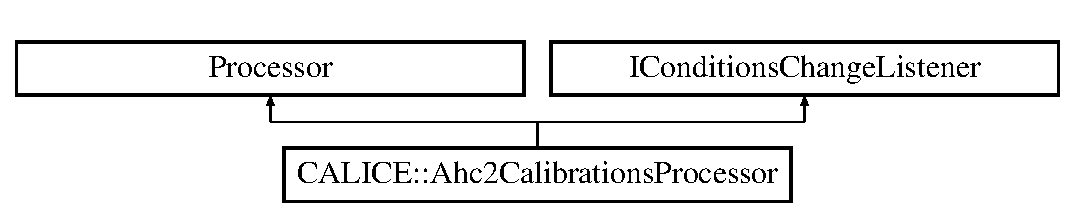
\includegraphics[height=2.000000cm]{classCALICE_1_1Ahc2CalibrationsProcessor}
\end{center}
\end{figure}
\subsection*{Public Member Functions}
\begin{DoxyCompactItemize}
\item 
virtual Processor $\ast$ {\bfseries new\-Processor} ()\label{classCALICE_1_1Ahc2CalibrationsProcessor_aa6634c358a285cfccf3c226e4b2aba44}

\item 
virtual void {\bfseries init} ()\label{classCALICE_1_1Ahc2CalibrationsProcessor_a51c5ec4099919e164ddbf819249c68f8}

\item 
virtual void {\bfseries process\-Event} (L\-C\-Event $\ast$evt)\label{classCALICE_1_1Ahc2CalibrationsProcessor_a0fa7ec48d16b46b6446dd7d44bcf718a}

\item 
virtual void {\bfseries end} ()\label{classCALICE_1_1Ahc2CalibrationsProcessor_a39d7ee9421e4859533f3d136e0b09c58}

\item 
virtual void {\bfseries conditions\-Changed} (L\-C\-Collection $\ast$col)\label{classCALICE_1_1Ahc2CalibrationsProcessor_ace470f4ce9130dfca7cac9319e4b2930}

\end{DoxyCompactItemize}
\subsection*{Static Public Member Functions}
\begin{DoxyCompactItemize}
\item 
static Mapped\-Container\\*
$<$ Ahc2\-Calibrations $>$ $\ast$ {\bf get\-Calibrations} (const std\-::string \&processor\-Name)
\begin{DoxyCompactList}\small\item\em static function to obtain a Mapped\-Container with cell neighbours \end{DoxyCompactList}\end{DoxyCompactItemize}
\subsection*{Private Member Functions}
\begin{DoxyCompactItemize}
\item 
void {\bfseries update\-Mapping} ()\label{classCALICE_1_1Ahc2CalibrationsProcessor_a657ac692143a138582df4586cfaebf7b}

\item 
void {\bfseries update\-M\-I\-P\-Calibration} ()\label{classCALICE_1_1Ahc2CalibrationsProcessor_ae53f7d493e2355d86f8ba57bf26b5e34}

\item 
void {\bfseries update\-Gain\-Calibration} ()\label{classCALICE_1_1Ahc2CalibrationsProcessor_a0b6289d487354620a8a79885c7979b48}

\item 
void {\bfseries update\-Pedestal} ()\label{classCALICE_1_1Ahc2CalibrationsProcessor_ac52f352570f32ee3df3b63fcf46891ac}

\item 
void {\bfseries update\-Low\-Gain\-Pedestal} ()\label{classCALICE_1_1Ahc2CalibrationsProcessor_a880a5ba65d6bfe9e7ff260b6db190fa1}

\item 
void {\bfseries update\-Pedestal\-Memory\-Cell\-Offset} ()\label{classCALICE_1_1Ahc2CalibrationsProcessor_aae98b664197540cc0068842de310ae7f}

\item 
void {\bfseries update\-Low\-Gain\-Pedestal\-Memory\-Cell\-Offset} ()\label{classCALICE_1_1Ahc2CalibrationsProcessor_adde02bccc6fc6f4705a3644b9c53199f}

\item 
void {\bfseries update\-Temperature} ()\label{classCALICE_1_1Ahc2CalibrationsProcessor_a46bc7e0dee10380b0e0aca96e62386e9}

\item 
void {\bfseries update\-Inter\-Calibration} ()\label{classCALICE_1_1Ahc2CalibrationsProcessor_a5f9c37499166c12365d6232b46c390a1}

\item 
void {\bfseries update\-Physics\-Calib\-I\-C} ()\label{classCALICE_1_1Ahc2CalibrationsProcessor_ad2b787969eddcf1c9ebb4446c3b36c32}

\item 
void {\bfseries update\-Saturation\-Parameters} ()\label{classCALICE_1_1Ahc2CalibrationsProcessor_a564b256fc9d0eb1b95028269f9e55853}

\item 
void {\bfseries update\-Time\-Slopes\-Parameters} ()\label{classCALICE_1_1Ahc2CalibrationsProcessor_a3922efdd9d5bec20724fb4ebec6d35a6}

\item 
void {\bfseries update\-Time\-Offset\-Parameters} ()\label{classCALICE_1_1Ahc2CalibrationsProcessor_a80bfc72b1b6d14ccddbd48a7a9bab8fd}

\item 
void {\bfseries update\-Time\-Offset\-Mem\-Cell\-Even\-Parameters} ()\label{classCALICE_1_1Ahc2CalibrationsProcessor_af7c510882ffaff05d91d581a095ed2ce}

\item 
void {\bfseries update\-Time\-Offset\-Mem\-Cell\-Odd\-Parameters} ()\label{classCALICE_1_1Ahc2CalibrationsProcessor_ab29ff09c1cb8b2ed092924e089ccfa4f}

\item 
void {\bfseries update\-Time\-Offset\-Mem\-Cell\-Even\-Buffer\-Even\-Event\-Even\-Parameters} ()\label{classCALICE_1_1Ahc2CalibrationsProcessor_a06824d23f67a292834fe3dec4a5865a8}

\item 
void {\bfseries update\-Time\-Offset\-Mem\-Cell\-Odd\-Buffer\-Even\-Event\-Odd\-Parameters} ()\label{classCALICE_1_1Ahc2CalibrationsProcessor_a4f9e888b8b80adbaed2fafc8f5246ea5}

\item 
void {\bfseries update\-Time\-Offset\-Mem\-Cell\-Even\-Buffer\-Odd\-Event\-Even\-Parameters} ()\label{classCALICE_1_1Ahc2CalibrationsProcessor_ac024962693135181be10780bdf49fd86}

\item 
void {\bfseries update\-Time\-Offset\-Mem\-Cell\-Odd\-Buffer\-Odd\-Event\-Odd\-Parameters} ()\label{classCALICE_1_1Ahc2CalibrationsProcessor_a994f55c48904be6d97d9c7e63ae68e93}

\item 
void {\bfseries update\-Occupancy\-Bxid\-Even\-High\-Gain\-Parameters} ()\label{classCALICE_1_1Ahc2CalibrationsProcessor_ae21d5ec42eaa934545d0250478471d0e}

\item 
void {\bfseries update\-Occupancy\-Bxid\-Even\-Low\-Gain\-Parameters} ()\label{classCALICE_1_1Ahc2CalibrationsProcessor_aa93e030e73b7d28b4e729bded9f7869a}

\item 
void {\bfseries update\-Occupancy\-Bxid\-Odd\-High\-Gain\-Parameters} ()\label{classCALICE_1_1Ahc2CalibrationsProcessor_a95e4ce302109eaab9b887c619c045c71}

\item 
void {\bfseries update\-Occupancy\-Bxid\-Odd\-Low\-Gain\-Parameters} ()\label{classCALICE_1_1Ahc2CalibrationsProcessor_ac3116911c9d038af272736216a716213}

\item 
void {\bfseries update\-Cell\-Quality} ()\label{classCALICE_1_1Ahc2CalibrationsProcessor_ab9278b6dd3733e2c48d85e76786960bd}

\item 
void {\bfseries update\-Module\-Encoding\-String\-From\-D\-B} (L\-C\-Collection $\ast$col, Decoder\-Set $\ast$decoder)\label{classCALICE_1_1Ahc2CalibrationsProcessor_ac210e973bf0996f2db99636c445b9191}

\item 
bool {\bfseries is\-Module\-Encoding\-String\-Valid} (std\-::string module\-Encoding\-String)\label{classCALICE_1_1Ahc2CalibrationsProcessor_ac5e275a92989804a26737ae527f38d03}

\end{DoxyCompactItemize}
\subsection*{Private Attributes}
\begin{DoxyCompactItemize}
\item 
Mapped\-Container\\*
$<$ Ahc2\-Calibrations $>$ $\ast$ {\bfseries \-\_\-container}\label{classCALICE_1_1Ahc2CalibrationsProcessor_aeaef0bab14c19834840e2633b4f5d858}

\item 
std\-::vector$<$ Ahc2\-Calibrations $\ast$ $>$ {\bfseries \-\_\-all\-Calibrations}\label{classCALICE_1_1Ahc2CalibrationsProcessor_ad412992a7bbd961b8336be89fcac337a}

\item 
std\-::string {\bfseries \-\_\-module\-Encoding\-String}\label{classCALICE_1_1Ahc2CalibrationsProcessor_a5b91132b3f78fc93e1c13d23df72b037}

\item 
std\-::string {\bfseries \-\_\-mapping\-Processor\-Name}\label{classCALICE_1_1Ahc2CalibrationsProcessor_a23d71b66f35914b756f49eb1e4aff6ef}

\item 
std\-::string {\bfseries \-\_\-\-E4\-D\-Mapper\-Col\-Name}\label{classCALICE_1_1Ahc2CalibrationsProcessor_ade555589de87ce42ad5dd8b31e84e25b}

\item 
std\-::string {\bfseries \-\_\-\-M\-I\-P\-Constant\-Col\-Name}\label{classCALICE_1_1Ahc2CalibrationsProcessor_a37f15328faa5231abb27b03b32d518f9}

\item 
std\-::string {\bfseries \-\_\-\-M\-I\-P\-Slope\-Col\-Name}\label{classCALICE_1_1Ahc2CalibrationsProcessor_a658922d38003bbfa9b3e272f21470533}

\item 
std\-::string {\bfseries \-\_\-gain\-Constant\-Col\-Name}\label{classCALICE_1_1Ahc2CalibrationsProcessor_a969e32fb8ce307d657440a5e079b63f0}

\item 
std\-::string {\bfseries \-\_\-gain\-Slope\-Col\-Name}\label{classCALICE_1_1Ahc2CalibrationsProcessor_af5870e7f9df7a9546cbe3f245d5c50aa}

\item 
std\-::string {\bfseries \-\_\-inter\-Calibration\-Col\-Name}\label{classCALICE_1_1Ahc2CalibrationsProcessor_a3d850731299639d9a1f9a13b4063a2f4}

\item 
std\-::string {\bfseries \-\_\-\-Physics\-Calib\-I\-C\-Col\-Name}\label{classCALICE_1_1Ahc2CalibrationsProcessor_aab920d306e59f70262c7d5eddae09e2f}

\item 
std\-::string {\bfseries \-\_\-pedestal\-Col\-Name}\label{classCALICE_1_1Ahc2CalibrationsProcessor_a1e096b845c6c4ec79fa9b55d8a836f63}

\item 
std\-::string {\bfseries \-\_\-low\-Gain\-Pedestal\-Col\-Name}\label{classCALICE_1_1Ahc2CalibrationsProcessor_a7a5b484a532ab700082a885f2ef85c4e}

\item 
std\-::string {\bfseries \-\_\-pedestal\-Memory\-Cell\-Offset\-Col\-Name}\label{classCALICE_1_1Ahc2CalibrationsProcessor_af954c57e514a1313cc4aeb4b17c8e698}

\item 
std\-::string {\bfseries \-\_\-low\-Gain\-Pedestal\-Memory\-Cell\-Offset\-Col\-Name}\label{classCALICE_1_1Ahc2CalibrationsProcessor_a546f9a5a91829338127c4e119e011388}

\item 
std\-::string {\bfseries \-\_\-temperature\-Col\-Name}\label{classCALICE_1_1Ahc2CalibrationsProcessor_a1550307968315d0308613e1840af70d7}

\item 
std\-::string {\bfseries \-\_\-saturation\-Parameters\-Col\-Name}\label{classCALICE_1_1Ahc2CalibrationsProcessor_ae71cd63d436ed4f645b13d1071411b01}

\item 
std\-::string {\bfseries \-\_\-time\-Slopes\-Parameters\-Col\-Name}\label{classCALICE_1_1Ahc2CalibrationsProcessor_a3c9a4f1c5e75c82e7e1e1a7a02c9dce1}

\item 
std\-::string {\bfseries \-\_\-time\-Offset\-Parameters\-Col\-Name}\label{classCALICE_1_1Ahc2CalibrationsProcessor_a35bb47e065ab2a711c7b2a1b20eb0877}

\item 
std\-::string {\bfseries \-\_\-time\-Offset\-Mem\-Cell\-Even\-Parameters\-Col\-Name}\label{classCALICE_1_1Ahc2CalibrationsProcessor_a59ae9442d7ebd3da64794c11ef0985f8}

\item 
std\-::string {\bfseries \-\_\-time\-Offset\-Mem\-Cell\-Odd\-Parameters\-Col\-Name}\label{classCALICE_1_1Ahc2CalibrationsProcessor_aef8f9816233d4ce9cb039cc1a1b1b627}

\item 
std\-::string {\bfseries \-\_\-time\-Offset\-Mem\-Cell\-Even\-Buffer\-Even\-Event\-Even\-Parameters\-Col\-Name}\label{classCALICE_1_1Ahc2CalibrationsProcessor_a234a134d3d68248033fadcfd9f1deff2}

\item 
std\-::string {\bfseries \-\_\-time\-Offset\-Mem\-Cell\-Odd\-Buffer\-Even\-Event\-Odd\-Parameters\-Col\-Name}\label{classCALICE_1_1Ahc2CalibrationsProcessor_a04b275eb495cb5604b231839a20283bc}

\item 
std\-::string {\bfseries \-\_\-time\-Offset\-Mem\-Cell\-Even\-Buffer\-Odd\-Event\-Even\-Parameters\-Col\-Name}\label{classCALICE_1_1Ahc2CalibrationsProcessor_ad7d7b17901f5c1b6e980bba81bc10c06}

\item 
std\-::string {\bfseries \-\_\-time\-Offset\-Mem\-Cell\-Odd\-Buffer\-Odd\-Event\-Odd\-Parameters\-Col\-Name}\label{classCALICE_1_1Ahc2CalibrationsProcessor_a5187ff2a965498fd93aff337fe1b68be}

\item 
std\-::string {\bfseries \-\_\-\-Occupancy\-Bxid\-Even\-High\-Gain\-Parameters\-Col\-Name}\label{classCALICE_1_1Ahc2CalibrationsProcessor_a79e8c84a537b73e02fd107abb892ffeb}

\item 
std\-::string {\bfseries \-\_\-\-Occupancy\-Bxid\-Even\-Low\-Gain\-Parameters\-Col\-Name}\label{classCALICE_1_1Ahc2CalibrationsProcessor_adb42513dab8255b1f1a9622070856823}

\item 
std\-::string {\bfseries \-\_\-\-Occupancy\-Bxid\-Odd\-High\-Gain\-Parameters\-Col\-Name}\label{classCALICE_1_1Ahc2CalibrationsProcessor_aae456e27f91ea369ab33937b53211b41}

\item 
std\-::string {\bfseries \-\_\-\-Occupancy\-Bxid\-Odd\-Low\-Gain\-Parameters\-Col\-Name}\label{classCALICE_1_1Ahc2CalibrationsProcessor_aa402b142c9b9c84024b97bc016e9d31b}

\item 
std\-::string {\bfseries \-\_\-cell\-Quality\-Col\-Name}\label{classCALICE_1_1Ahc2CalibrationsProcessor_a4f86dc624210d2b80067a267f2112367}

\item 
L\-C\-Collection $\ast$ {\bfseries \-\_\-\-E4\-D\-Mapper\-Col}\label{classCALICE_1_1Ahc2CalibrationsProcessor_a8e5253174aabd0ebebf8a7d709e0b43e}

\item 
L\-C\-Collection $\ast$ {\bfseries \-\_\-\-M\-I\-P\-Constant\-Col}\label{classCALICE_1_1Ahc2CalibrationsProcessor_a5ec3439e0a6716a3262510e678f98789}

\item 
L\-C\-Collection $\ast$ {\bfseries \-\_\-\-M\-I\-P\-Slope\-Col}\label{classCALICE_1_1Ahc2CalibrationsProcessor_addc2a8fe5bff9b7b16ddc50bd8fdb245}

\item 
L\-C\-Collection $\ast$ {\bfseries \-\_\-gain\-Constant\-Col}\label{classCALICE_1_1Ahc2CalibrationsProcessor_a74e33507c5f4d7d9b16603835d381ef0}

\item 
L\-C\-Collection $\ast$ {\bfseries \-\_\-gain\-Slope\-Col}\label{classCALICE_1_1Ahc2CalibrationsProcessor_af9303081cdaa45e793dbb5c4ed68c933}

\item 
L\-C\-Collection $\ast$ {\bfseries \-\_\-inter\-Calibration\-Col}\label{classCALICE_1_1Ahc2CalibrationsProcessor_a572c6374b74c9d250dbdb0abf109595d}

\item 
L\-C\-Collection $\ast$ {\bfseries \-\_\-\-Physics\-Calib\-I\-C\-Col}\label{classCALICE_1_1Ahc2CalibrationsProcessor_a7534c9d91bbb0c58f135e69384344f37}

\item 
L\-C\-Collection $\ast$ {\bfseries \-\_\-pedestal\-Col}\label{classCALICE_1_1Ahc2CalibrationsProcessor_ae150a0d45e11c2c4f6ce07f479ada8b0}

\item 
L\-C\-Collection $\ast$ {\bfseries \-\_\-low\-Gain\-Pedestal\-Col}\label{classCALICE_1_1Ahc2CalibrationsProcessor_a785a8f5c067d4eec82e91c50f3be343b}

\item 
L\-C\-Collection $\ast$ {\bfseries \-\_\-pedestal\-Memory\-Cell\-Offset\-Col}\label{classCALICE_1_1Ahc2CalibrationsProcessor_a72e27f1de40abe570d78b435d59e237f}

\item 
L\-C\-Collection $\ast$ {\bfseries \-\_\-low\-Gain\-Pedestal\-Memory\-Cell\-Offset\-Col}\label{classCALICE_1_1Ahc2CalibrationsProcessor_a2dc98afc06490e6e3b210833b67f05d3}

\item 
L\-C\-Collection $\ast$ {\bfseries \-\_\-temperature\-Col}\label{classCALICE_1_1Ahc2CalibrationsProcessor_aa219003f8cbfe58b6bf9b45ee9636437}

\item 
L\-C\-Collection $\ast$ {\bfseries \-\_\-saturation\-Parameters\-Col}\label{classCALICE_1_1Ahc2CalibrationsProcessor_a306a43df8fc9cb84c4e4069ff7c8d2f1}

\item 
L\-C\-Collection $\ast$ {\bfseries \-\_\-time\-Slopes\-Parameters\-Col}\label{classCALICE_1_1Ahc2CalibrationsProcessor_a611275318f6e7ad6799eac941b3b4d6b}

\item 
L\-C\-Collection $\ast$ {\bfseries \-\_\-time\-Offset\-Parameters\-Col}\label{classCALICE_1_1Ahc2CalibrationsProcessor_acbfec942e148883b15ce206992cb2f1f}

\item 
L\-C\-Collection $\ast$ {\bfseries \-\_\-time\-Offset\-Mem\-Cell\-Even\-Parameters\-Col}\label{classCALICE_1_1Ahc2CalibrationsProcessor_a71e971985c7b37ac0202b3a338ad854a}

\item 
L\-C\-Collection $\ast$ {\bfseries \-\_\-time\-Offset\-Mem\-Cell\-Odd\-Parameters\-Col}\label{classCALICE_1_1Ahc2CalibrationsProcessor_afbf3fec4d9ce36c1c9c5e76193085f4b}

\item 
L\-C\-Collection $\ast$ {\bfseries \-\_\-time\-Offset\-Mem\-Cell\-Even\-Buffer\-Even\-Event\-Even\-Parameters\-Col}\label{classCALICE_1_1Ahc2CalibrationsProcessor_aa21eb1278283dacd26bcf05716700d26}

\item 
L\-C\-Collection $\ast$ {\bfseries \-\_\-time\-Offset\-Mem\-Cell\-Odd\-Buffer\-Even\-Event\-Odd\-Parameters\-Col}\label{classCALICE_1_1Ahc2CalibrationsProcessor_ae44b5d30d19f65a658380340b25e1e90}

\item 
L\-C\-Collection $\ast$ {\bfseries \-\_\-time\-Offset\-Mem\-Cell\-Even\-Buffer\-Odd\-Event\-Even\-Parameters\-Col}\label{classCALICE_1_1Ahc2CalibrationsProcessor_aae89f20dd3332110abeefaee429fab36}

\item 
L\-C\-Collection $\ast$ {\bfseries \-\_\-time\-Offset\-Mem\-Cell\-Odd\-Buffer\-Odd\-Event\-Odd\-Parameters\-Col}\label{classCALICE_1_1Ahc2CalibrationsProcessor_a5c96aed5a622dc2c6deb32b5b5426f5e}

\item 
L\-C\-Collection $\ast$ {\bfseries \-\_\-\-Occupancy\-Bxid\-Even\-High\-Gain\-Parameters\-Col}\label{classCALICE_1_1Ahc2CalibrationsProcessor_a5155ec83b6865e7f728a4f05e582025c}

\item 
L\-C\-Collection $\ast$ {\bfseries \-\_\-\-Occupancy\-Bxid\-Even\-Low\-Gain\-Parameters\-Col}\label{classCALICE_1_1Ahc2CalibrationsProcessor_aabd876ae2bef96e85a61c3655f47224b}

\item 
L\-C\-Collection $\ast$ {\bfseries \-\_\-\-Occupancy\-Bxid\-Odd\-High\-Gain\-Parameters\-Col}\label{classCALICE_1_1Ahc2CalibrationsProcessor_abbdaa7b95bd8505ff644b46d80f25727}

\item 
L\-C\-Collection $\ast$ {\bfseries \-\_\-\-Occupancy\-Bxid\-Odd\-Low\-Gain\-Parameters\-Col}\label{classCALICE_1_1Ahc2CalibrationsProcessor_a1ee40e1eda4e4b01f6050b9a450d8935}

\item 
L\-C\-Collection $\ast$ {\bfseries \-\_\-cell\-Quality\-Col}\label{classCALICE_1_1Ahc2CalibrationsProcessor_af5eee39f06b27a9f3ebb9a82705b05f9}

\item 
bool {\bfseries \-\_\-\-E4\-D\-Mapper\-Changed}\label{classCALICE_1_1Ahc2CalibrationsProcessor_a0849fba95890f27f0875320c5da5ea06}

\item 
bool {\bfseries \-\_\-\-M\-I\-P\-Constant\-Changed}\label{classCALICE_1_1Ahc2CalibrationsProcessor_ae940128be9e0e2554a1042034f726f3a}

\item 
bool {\bfseries \-\_\-\-M\-I\-P\-Slope\-Changed}\label{classCALICE_1_1Ahc2CalibrationsProcessor_ac2f78af7fb5676854f860e818da02bd5}

\item 
bool {\bfseries \-\_\-gain\-Constant\-Changed}\label{classCALICE_1_1Ahc2CalibrationsProcessor_a61a4ef1b69de5196205e6c4daa9f31a5}

\item 
bool {\bfseries \-\_\-gain\-Slope\-Changed}\label{classCALICE_1_1Ahc2CalibrationsProcessor_afc35c0f92c08eeffcfe941a429c1fe71}

\item 
bool {\bfseries \-\_\-inter\-Calibration\-Changed}\label{classCALICE_1_1Ahc2CalibrationsProcessor_ab855dae51cc8647606b0cf6fdc2a191e}

\item 
bool {\bfseries \-\_\-\-Physics\-Calib\-I\-C\-Changed}\label{classCALICE_1_1Ahc2CalibrationsProcessor_abaafd4c212b1b401f6553fb2944e82e5}

\item 
bool {\bfseries \-\_\-pedestal\-Changed}\label{classCALICE_1_1Ahc2CalibrationsProcessor_a42022638b9b84f13b786c64885a1c9f6}

\item 
bool {\bfseries \-\_\-low\-Gain\-Pedestal\-Changed}\label{classCALICE_1_1Ahc2CalibrationsProcessor_a880c0a6fffff1a87e6257b89be25a21e}

\item 
bool {\bfseries \-\_\-pedestal\-Memory\-Cell\-Offset\-Changed}\label{classCALICE_1_1Ahc2CalibrationsProcessor_ae65f258dd5f3962aa82a4941ee911ff2}

\item 
bool {\bfseries \-\_\-low\-Gain\-Pedestal\-Memory\-Cell\-Offset\-Changed}\label{classCALICE_1_1Ahc2CalibrationsProcessor_a84bac84c7832403d07096b039ea97f8c}

\item 
bool {\bfseries \-\_\-temperature\-Changed}\label{classCALICE_1_1Ahc2CalibrationsProcessor_a5c90fad3b22edd95242ee34abc0ab388}

\item 
bool {\bfseries \-\_\-saturation\-Parameters\-Changed}\label{classCALICE_1_1Ahc2CalibrationsProcessor_a9bdd269df77282d9c8e6b4c77f604475}

\item 
bool {\bfseries \-\_\-time\-Slopes\-Parameters\-Changed}\label{classCALICE_1_1Ahc2CalibrationsProcessor_a498dd9b3fa8b2f48d12adb19fdcd6c3b}

\item 
bool {\bfseries \-\_\-time\-Offset\-Parameters\-Changed}\label{classCALICE_1_1Ahc2CalibrationsProcessor_ac1a042b7dc8892fd5648d2113734249b}

\item 
bool {\bfseries \-\_\-time\-Offset\-Mem\-Cell\-Even\-Parameters\-Changed}\label{classCALICE_1_1Ahc2CalibrationsProcessor_ac8d7b82d0fa4fb5ea6a72e93305c495c}

\item 
bool {\bfseries \-\_\-time\-Offset\-Mem\-Cell\-Odd\-Parameters\-Changed}\label{classCALICE_1_1Ahc2CalibrationsProcessor_a90b8afc94256ac4bb6a4a2f1f191f303}

\item 
bool {\bfseries \-\_\-time\-Offset\-Mem\-Cell\-Even\-Buffer\-Even\-Event\-Even\-Parameters\-Col\-Changed}\label{classCALICE_1_1Ahc2CalibrationsProcessor_a37aa455c8ae4e2593b7212c7d1822820}

\item 
bool {\bfseries \-\_\-time\-Offset\-Mem\-Cell\-Odd\-Buffer\-Even\-Event\-Odd\-Parameters\-Col\-Changed}\label{classCALICE_1_1Ahc2CalibrationsProcessor_adf951c1986d3f21c25c0a537c5b5e91f}

\item 
bool {\bfseries \-\_\-time\-Offset\-Mem\-Cell\-Even\-Buffer\-Odd\-Event\-Even\-Parameters\-Col\-Changed}\label{classCALICE_1_1Ahc2CalibrationsProcessor_a294f01498a84477c5e0269fd5aecc650}

\item 
bool {\bfseries \-\_\-time\-Offset\-Mem\-Cell\-Odd\-Buffer\-Odd\-Event\-Odd\-Parameters\-Col\-Changed}\label{classCALICE_1_1Ahc2CalibrationsProcessor_ae12569fa4ba2e497055985d2ed8cadfc}

\item 
bool {\bfseries \-\_\-\-Occupancy\-Bxid\-Even\-High\-Gain\-Parameters\-Col\-Changed}\label{classCALICE_1_1Ahc2CalibrationsProcessor_ae5daa0b7715aae1bc5060ab55682cbc2}

\item 
bool {\bfseries \-\_\-\-Occupancy\-Bxid\-Even\-Low\-Gain\-Parameters\-Col\-Changed}\label{classCALICE_1_1Ahc2CalibrationsProcessor_a8c4f0548a6f4a4fb79907ff157a37d73}

\item 
bool {\bfseries \-\_\-\-Occupancy\-Bxid\-Odd\-High\-Gain\-Parameters\-Col\-Changed}\label{classCALICE_1_1Ahc2CalibrationsProcessor_af0fa9255b41292d3e7f79f8d58e57b09}

\item 
bool {\bfseries \-\_\-\-Occupancy\-Bxid\-Odd\-Low\-Gain\-Parameters\-Col\-Changed}\label{classCALICE_1_1Ahc2CalibrationsProcessor_ac61e9964bf68140d3a98d05b39c0bc73}

\item 
bool {\bfseries \-\_\-cell\-Quality\-Changed}\label{classCALICE_1_1Ahc2CalibrationsProcessor_af2fe562a0bc8eabc864c8ea71b8d93d4}

\item 
float {\bfseries \-\_\-global\-Pixel\-Scale\-Factor}\label{classCALICE_1_1Ahc2CalibrationsProcessor_ae0013a828607f480c2575fe6a25b2c52}

\item 
bool {\bfseries \-\_\-\-M\-I\-P\-Constant\-Scaled}\label{classCALICE_1_1Ahc2CalibrationsProcessor_ac36a61c2c1f52fe36b17a0b158d03e69}

\item 
bool {\bfseries \-\_\-\-M\-I\-P\-Slope\-Scaled}\label{classCALICE_1_1Ahc2CalibrationsProcessor_af5e80fad34c209c1765b80486762e012}

\item 
bool {\bfseries \-\_\-gain\-Constant\-Scaled}\label{classCALICE_1_1Ahc2CalibrationsProcessor_a6db8f6f1b1f26f5ec71e0a160b7b4cad}

\item 
bool {\bfseries \-\_\-gain\-Slope\-Scaled}\label{classCALICE_1_1Ahc2CalibrationsProcessor_a14fd7b81ea366e9c812e557ea53b8c54}

\item 
bool {\bfseries \-\_\-inter\-Calibration\-Scaled}\label{classCALICE_1_1Ahc2CalibrationsProcessor_a17c3b220c769b795d7a1a94af6a3c5fd}

\item 
bool {\bfseries \-\_\-\-Physics\-Calib\-I\-C\-Scaled}\label{classCALICE_1_1Ahc2CalibrationsProcessor_a61a602f7adbf9d3a0b20efa5d1fc623f}

\item 
float {\bfseries \-\_\-\-M\-I\-P\-Constant\-Scale\-Factor}\label{classCALICE_1_1Ahc2CalibrationsProcessor_a888e81f95e2371e85123739eda30e3f3}

\item 
float {\bfseries \-\_\-\-M\-I\-P\-Slope\-Scale\-Factor}\label{classCALICE_1_1Ahc2CalibrationsProcessor_a43d3f25063cf1681f3b92b26c87f3c84}

\item 
float {\bfseries \-\_\-gain\-Constant\-Scale\-Factor}\label{classCALICE_1_1Ahc2CalibrationsProcessor_a76055de9faebcfd1c46406293c218779}

\item 
float {\bfseries \-\_\-gain\-Slope\-Scale\-Factor}\label{classCALICE_1_1Ahc2CalibrationsProcessor_a956b9241e62ac83ceee8c9fd87fb2017}

\item 
float {\bfseries \-\_\-inter\-Calibration\-Scale\-Factor}\label{classCALICE_1_1Ahc2CalibrationsProcessor_a4de92b2ef11f86dff4cb1a789fa05e47}

\item 
float {\bfseries \-\_\-\-Physics\-Calib\-I\-C\-Scale\-Factor}\label{classCALICE_1_1Ahc2CalibrationsProcessor_ac14aa96530dd469d1b991affd9eaccee}

\item 
const Mapper $\ast$ {\bfseries \-\_\-mapper}\label{classCALICE_1_1Ahc2CalibrationsProcessor_a6f062e170f84713ec8f4e06507093e44}

\item 
unsigned int {\bfseries \-\_\-mapper\-Version}\label{classCALICE_1_1Ahc2CalibrationsProcessor_a6b3a5423f070321bf660836f352c15e6}

\end{DoxyCompactItemize}
\subsection*{Static Private Attributes}
\begin{DoxyCompactItemize}
\item 
static std\-::map$<$ std\-::string, \\*
Mapped\-Container\\*
$<$ Ahc2\-Calibrations $>$ $\ast$ $>$ {\bfseries \-\_\-\-Ahc2\-Calibrations\-Container\-Map}\label{classCALICE_1_1Ahc2CalibrationsProcessor_add637c60e0d65cc1f405cc13dae113bd}

\end{DoxyCompactItemize}


\subsection{Detailed Description}
Processor that provides Ahc2 prototype calibration information to other processors. 

To obtain the object in other processors use\-: \doxyref{Ahc2\-Calibrations\-Processor\-::get\-Calibrations}{p.}{classCALICE_1_1Ahc2CalibrationsProcessor_ae40adce445cfbd5dc4f426b1b99b9d8b}( \char`\"{}\-Ahc2\-Si\-P\-M\-Calibrations processor name\char`\"{} )

\begin{DoxyParagraph}{processor parameters}
\begin{TabularC}{2}
\hline
steering file parameter name &description  \\\cline{1-2}
{\bfseries {\itshape  Mapping\-Processor\-Name }}&name of the mapping processor that provides the necessary Mapper class \\\cline{1-2}
{\bfseries {\itshape  Mip\-Constant\-Collection }}&name of the M\-I\-P constants collection \\\cline{1-2}
{\bfseries {\itshape  Mip\-Slopes\-Collection }}&name of the M\-I\-P slopes collection \\\cline{1-2}
{\bfseries {\itshape  Gain\-Constant\-Collection }}&name of the gain constants collection \\\cline{1-2}
{\bfseries {\itshape  Gain\-Slope\-Collection }}&name of the gain slopes collection \\\cline{1-2}
{\bfseries {\itshape  Pedestal\-Collection }}&name of the pedestal collection \\\cline{1-2}
{\bfseries {\itshape  Saturation\-Parameters\-Collection }}&name of the saturation parameters collection \\\cline{1-2}
{\bfseries {\itshape  Time\-Slopes\-Parameters\-Collection }}&name of the timeslopes parameters collection \\\cline{1-2}
{\bfseries {\itshape  Time\-Ped\-Parameters\-Collection }}&name of the time pedestal parameters collection$<$/tr \\\cline{1-2}
{\bfseries {\itshape  Pixel\-Scale\-Factors\-Collection }}&name of the pixel scale factors collection \\\cline{1-2}
{\bfseries {\itshape  Global\-Pixel\-Scale\-Factor }}&global value for the pixel scale factor \\\cline{1-2}
{\bfseries {\itshape  Cell\-Quality\-Collection }}&name of the saturation collection \\\cline{1-2}
\end{TabularC}

\end{DoxyParagraph}
\begin{DoxyAuthor}{Author}
{\tt Shaojun.\-lu@desy.\-de} 
\end{DoxyAuthor}
\begin{DoxyVersion}{Version}
0.\-1 
\end{DoxyVersion}
\begin{DoxyDate}{Date}
January 2013 
\end{DoxyDate}


Definition at line 57 of file Ahc2\-Calibrations\-Processor.\-hh.



\subsection{Member Function Documentation}
\index{C\-A\-L\-I\-C\-E\-::\-Ahc2\-Calibrations\-Processor@{C\-A\-L\-I\-C\-E\-::\-Ahc2\-Calibrations\-Processor}!get\-Calibrations@{get\-Calibrations}}
\index{get\-Calibrations@{get\-Calibrations}!CALICE::Ahc2CalibrationsProcessor@{C\-A\-L\-I\-C\-E\-::\-Ahc2\-Calibrations\-Processor}}
\subsubsection[{get\-Calibrations}]{\setlength{\rightskip}{0pt plus 5cm}Mapped\-Container$<$ Ahc2\-Calibrations $>$ $\ast$ C\-A\-L\-I\-C\-E\-::\-Ahc2\-Calibrations\-Processor\-::get\-Calibrations (
\begin{DoxyParamCaption}
\item[{const std\-::string \&}]{processor\-Name}
\end{DoxyParamCaption}
)\hspace{0.3cm}{\ttfamily [static]}}\label{classCALICE_1_1Ahc2CalibrationsProcessor_ae40adce445cfbd5dc4f426b1b99b9d8b}


static function to obtain a Mapped\-Container with cell neighbours 


\begin{DoxyParams}[1]{Parameters}
\mbox{\tt in}  & {\em processor\-Name} & name of the \doxyref{Ahc2\-Calibrations\-Processor}{p.}{classCALICE_1_1Ahc2CalibrationsProcessor} that takes care of this Ahc2\-Calibrations. \\
\hline
\end{DoxyParams}
\begin{DoxyReturn}{Returns}
pointer to the Mapped\-Container including Si\-P\-M\-Calibrations 
\end{DoxyReturn}


Definition at line 36 of file Ahc2\-Calibrations\-Processor.\-cc.



The documentation for this class was generated from the following files\-:\begin{DoxyCompactItemize}
\item 
Ahc2\-Calibrations\-Processor.\-hh\item 
Ahc2\-Calibrations\-Processor.\-cc\end{DoxyCompactItemize}

\section{C\-A\-L\-I\-C\-E\-:\-:Pedestal\-Processor Class Reference}
\label{classCALICE_1_1PedestalProcessor}\index{C\-A\-L\-I\-C\-E\-::\-Pedestal\-Processor@{C\-A\-L\-I\-C\-E\-::\-Pedestal\-Processor}}


Processor which calculates the pedestals from pedestal events and writes them as a collection of Simple\-Value.  




{\ttfamily \#include $<$Pedestal\-Processor.\-hh$>$}

Inheritance diagram for C\-A\-L\-I\-C\-E\-:\-:Pedestal\-Processor\-:\begin{figure}[H]
\begin{center}
\leavevmode
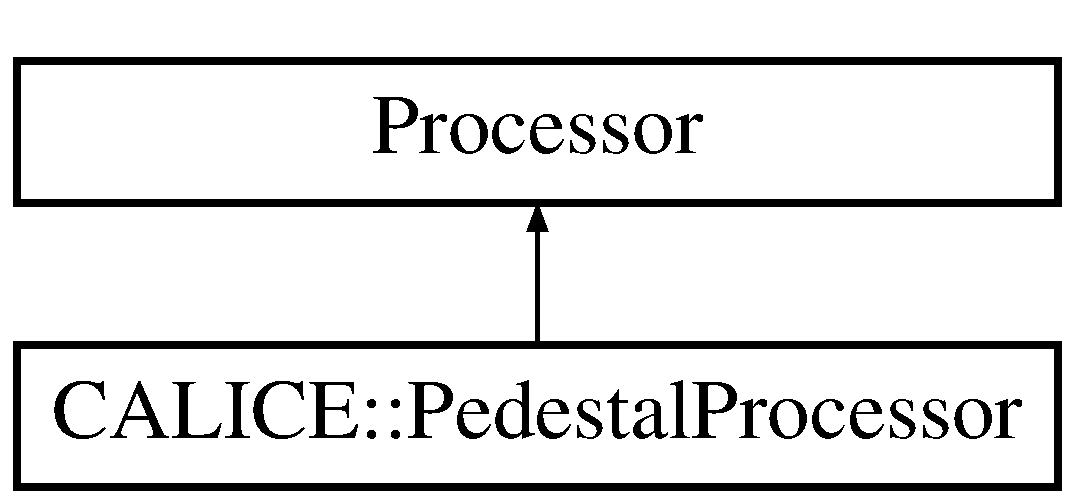
\includegraphics[height=2.000000cm]{classCALICE_1_1PedestalProcessor}
\end{center}
\end{figure}
\subsection*{Public Member Functions}
\begin{DoxyCompactItemize}
\item 
{\bf Pedestal\-Processor} ()\label{classCALICE_1_1PedestalProcessor_a6bc9bd585510a41c6ca0f563ef93e60d}

\begin{DoxyCompactList}\small\item\em Default constructor. \end{DoxyCompactList}\item 
{\bf $\sim$\-Pedestal\-Processor} ()\label{classCALICE_1_1PedestalProcessor_a7afefac07d219138d0cbb0a172292584}

\begin{DoxyCompactList}\small\item\em Destructor. \end{DoxyCompactList}\item 
{\bf Pedestal\-Processor} $\ast$ {\bf new\-Processor} ()\label{classCALICE_1_1PedestalProcessor_aaf59f11eb0d6cb2fd57e4093b2174edd}

\begin{DoxyCompactList}\small\item\em Return new instance of this processor. \end{DoxyCompactList}\item 
virtual void {\bf init} ()\label{classCALICE_1_1PedestalProcessor_a936b946a56f3e0c6203f413161d0b534}

\begin{DoxyCompactList}\small\item\em Initialise necessary variables. \end{DoxyCompactList}\item 
void {\bf process\-Event} (L\-C\-Event $\ast$evt)
\begin{DoxyCompactList}\small\item\em Process event (the working horse) \end{DoxyCompactList}\item 
virtual void {\bf end} ()\label{classCALICE_1_1PedestalProcessor_ace047025eb794a92d3abbfd089eb6b2c}

\begin{DoxyCompactList}\small\item\em Function called at the end of all events, for cleanup. \end{DoxyCompactList}\end{DoxyCompactItemize}
\subsection*{Protected Member Functions}
\begin{DoxyCompactItemize}
\item 
void {\bf update\-Mapper} ()\label{classCALICE_1_1PedestalProcessor_a3efefa4461047861ad09e26ff06c47ff}

\begin{DoxyCompactList}\small\item\em Update the mapper. \end{DoxyCompactList}\end{DoxyCompactItemize}
\subsection*{Protected Attributes}
\begin{DoxyCompactItemize}
\item 
std\-::string {\bf \-\_\-input\-Col\-Name}\label{classCALICE_1_1PedestalProcessor_ae7ff5ea5be5525611f209b13adcd7cee}

\begin{DoxyCompactList}\small\item\em name of the input collection \end{DoxyCompactList}\item 
std\-::string {\bf \-\_\-output\-Col\-Name}\label{classCALICE_1_1PedestalProcessor_aae6d1d5e7b01e107d18f2005d893e0ca}

\begin{DoxyCompactList}\small\item\em name of the output collection \end{DoxyCompactList}\item 
std\-::string {\bf \-\_\-mapping\-Processor\-Name}\label{classCALICE_1_1PedestalProcessor_a2dcdb3d16775dc1b4238d07a6bc27f6f}

\begin{DoxyCompactList}\small\item\em name of the processor providing the mapper \end{DoxyCompactList}\item 
Trigger\-Bits {\bfseries \-\_\-trigger\-Conf}\label{classCALICE_1_1PedestalProcessor_a1cf8086fe463615886f57f0b5be05d82}

\item 
int {\bf \-\_\-min\-Ped\-Number}\label{classCALICE_1_1PedestalProcessor_af438d9894110cd623ef6d95425a5459c}

\begin{DoxyCompactList}\small\item\em minimum number of events for which pedestal should be calculated \end{DoxyCompactList}\item 
int {\bf \-\_\-update\-Frequency}\label{classCALICE_1_1PedestalProcessor_a10205895bc6b3368876faf742beb5581}

\begin{DoxyCompactList}\small\item\em frequency with which the pedestal should be calculated \end{DoxyCompactList}\item 
int {\bf \-\_\-ped\-Counter}\label{classCALICE_1_1PedestalProcessor_a7ab871cec6528446d963c8d828abe0b9}

\begin{DoxyCompactList}\small\item\em counter for the number of pedestal events \end{DoxyCompactList}\item 
bool {\bf \-\_\-skip\-Minimum\-Event}\label{classCALICE_1_1PedestalProcessor_af2eb3cdd7d27a5033bfd669661e61697}

\begin{DoxyCompactList}\small\item\em flag to skip a min\-Ped\-Number of events \end{DoxyCompactList}\item 
const Ahc\-Mapper $\ast$ {\bf \-\_\-mapper}\label{classCALICE_1_1PedestalProcessor_ae5162fd017ae4a1abb03921d3bb3bfba}

\begin{DoxyCompactList}\small\item\em the mapper \end{DoxyCompactList}\item 
unsigned int {\bf \-\_\-mapper\-Version}\label{classCALICE_1_1PedestalProcessor_aef19163d8be045f83115d034221a3489}

\begin{DoxyCompactList}\small\item\em the mapper version (which changes when the mapper changes) \end{DoxyCompactList}\item 
L\-C\-Collection $\ast$ {\bf \-\_\-col\-Pedestal}\label{classCALICE_1_1PedestalProcessor_ab0c600b05c496702970da836d970cd48}

\begin{DoxyCompactList}\small\item\em collection with pedestal events \end{DoxyCompactList}\item 
Run\-Time\-Conditions\-Handler $\ast$ {\bf \-\_\-conditions\-Handler}\label{classCALICE_1_1PedestalProcessor_a3a39a6ea9341d4a6595227bc3947b4ac}

\begin{DoxyCompactList}\small\item\em pointer to the run time conditions handler \end{DoxyCompactList}\item 
float $\ast$$\ast$ {\bf \-\_\-ped\-Sum}\label{classCALICE_1_1PedestalProcessor_a7659ed593bf1fa8c4d6fea3332976765}

\begin{DoxyCompactList}\small\item\em double array of [module][cell] for the pedestal sum \end{DoxyCompactList}\item 
float $\ast$$\ast$ {\bf \-\_\-ped\-Sum\-Square}\label{classCALICE_1_1PedestalProcessor_a9e0ddd7ae0bba557fd530741f6d386e5}

\begin{DoxyCompactList}\small\item\em double array of [module][cell] for the pedestal sum squared \end{DoxyCompactList}\item 
unsigned int $\ast$$\ast$ {\bf \-\_\-ped\-Num}\label{classCALICE_1_1PedestalProcessor_a9460997dc6fe25a8e362a93b20bc3ef9}

\begin{DoxyCompactList}\small\item\em double array of [module][cell] for the number of pedestal events \end{DoxyCompactList}\item 
float $\ast$$\ast$ {\bf \-\_\-ped}\label{classCALICE_1_1PedestalProcessor_a90da1932accfd689ab713b4cc576ee6d}

\begin{DoxyCompactList}\small\item\em double array of [module][cell] for the pedestal value \end{DoxyCompactList}\item 
float $\ast$$\ast$ {\bf \-\_\-ped\-Error}\label{classCALICE_1_1PedestalProcessor_a127197da1199d8cecd356718609616e8}

\begin{DoxyCompactList}\small\item\em double array of [module][cell] for the pedestal error \end{DoxyCompactList}\item 
unsigned int {\bf \-\_\-ahc\-Max\-Number\-Of\-Modules}\label{classCALICE_1_1PedestalProcessor_a476f3cc6d6a29482ec95e2fd3d84081e}

\begin{DoxyCompactList}\small\item\em A\-H\-C\-A\-L maximum number of modules (39) \end{DoxyCompactList}\item 
unsigned int {\bf \-\_\-ahc\-Max\-Number\-Of\-Channels}\label{classCALICE_1_1PedestalProcessor_a48806ad75d6e2d07b74b94983f3b0c8b}

\begin{DoxyCompactList}\small\item\em A\-H\-C\-A\-L maximum number of channels. \end{DoxyCompactList}\item 
unsigned int {\bf \-\_\-ahc\-Max\-Number\-Of\-Chips}\label{classCALICE_1_1PedestalProcessor_ab39bcf808bee762e209218547e4e8e3b}

\begin{DoxyCompactList}\small\item\em A\-H\-C\-A\-L maximum number of chips. \end{DoxyCompactList}\item 
unsigned int {\bf \-\_\-ahc\-Max\-Number\-Of\-Cells}\label{classCALICE_1_1PedestalProcessor_ab6b7f92f8127ddf820ce1463f4870457}

\begin{DoxyCompactList}\small\item\em A\-H\-C\-A\-L maximum number of cells. \end{DoxyCompactList}\end{DoxyCompactItemize}


\subsection{Detailed Description}
Processor which calculates the pedestals from pedestal events and writes them as a collection of Simple\-Value. 

Note that the pedestal is the average energy (in A\-D\-C counts) of all pedestal hits. \begin{DoxyAuthor}{Author}
{\tt angela-\/isabela.\-lucaci-\/timoce@desy.\-de} 
\end{DoxyAuthor}
\begin{DoxyDate}{Date}
Dec 2009 
\end{DoxyDate}


Definition at line 21 of file Pedestal\-Processor.\-hh.



\subsection{Member Function Documentation}
\index{C\-A\-L\-I\-C\-E\-::\-Pedestal\-Processor@{C\-A\-L\-I\-C\-E\-::\-Pedestal\-Processor}!process\-Event@{process\-Event}}
\index{process\-Event@{process\-Event}!CALICE::PedestalProcessor@{C\-A\-L\-I\-C\-E\-::\-Pedestal\-Processor}}
\subsubsection[{process\-Event}]{\setlength{\rightskip}{0pt plus 5cm}void C\-A\-L\-I\-C\-E\-::\-Pedestal\-Processor\-::process\-Event (
\begin{DoxyParamCaption}
\item[{L\-C\-Event $\ast$}]{evt}
\end{DoxyParamCaption}
)}\label{classCALICE_1_1PedestalProcessor_a38b604fcbf248fd117ad099d080e4b9f}


Process event (the working horse) 


\begin{DoxyParams}{Parameters}
{\em evt} & event to be processed \\
\hline
\end{DoxyParams}


Definition at line 160 of file Pedestal\-Processor.\-cc.



References \-\_\-ahc\-Max\-Number\-Of\-Cells, \-\_\-ahc\-Max\-Number\-Of\-Chips, \-\_\-ahc\-Max\-Number\-Of\-Modules, \-\_\-col\-Pedestal, \-\_\-conditions\-Handler, \-\_\-input\-Col\-Name, \-\_\-mapper, \-\_\-mapper\-Version, \-\_\-min\-Ped\-Number, \-\_\-ped, \-\_\-ped\-Counter, \-\_\-ped\-Error, \-\_\-ped\-Num, \-\_\-ped\-Sum, \-\_\-ped\-Sum\-Square, \-\_\-skip\-Minimum\-Event, and update\-Mapper().



The documentation for this class was generated from the following files\-:\begin{DoxyCompactItemize}
\item 
Pedestal\-Processor.\-hh\item 
Pedestal\-Processor.\-cc\end{DoxyCompactItemize}

\section{C\-A\-L\-I\-C\-E\-:\-:Si\-P\-M\-Calibrate\-Processor Class Reference}
\label{classCALICE_1_1SiPMCalibrateProcessor}\index{C\-A\-L\-I\-C\-E\-::\-Si\-P\-M\-Calibrate\-Processor@{C\-A\-L\-I\-C\-E\-::\-Si\-P\-M\-Calibrate\-Processor}}


Processor that does the Si\-P\-M calibration.  




{\ttfamily \#include $<$Si\-P\-M\-Calibrate\-Processor.\-hh$>$}

Inheritance diagram for C\-A\-L\-I\-C\-E\-:\-:Si\-P\-M\-Calibrate\-Processor\-:\begin{figure}[H]
\begin{center}
\leavevmode
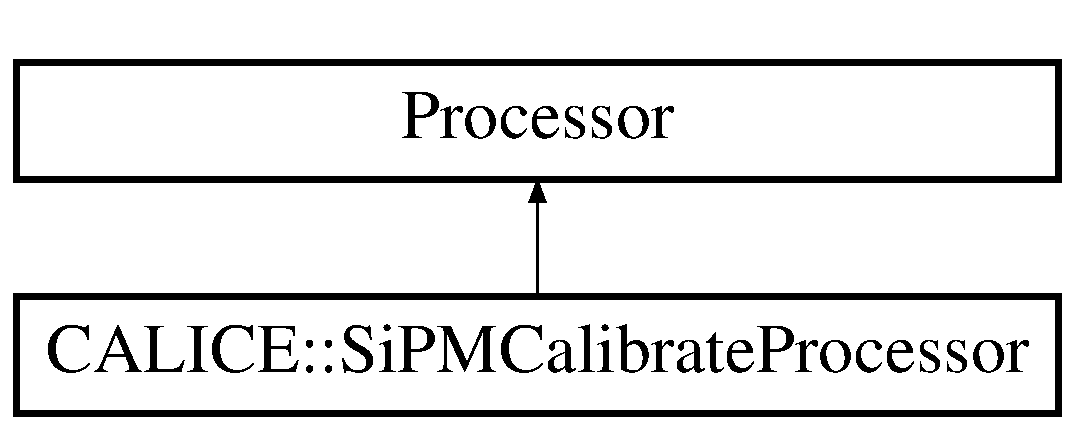
\includegraphics[height=2.000000cm]{classCALICE_1_1SiPMCalibrateProcessor}
\end{center}
\end{figure}
\subsection*{Public Member Functions}
\begin{DoxyCompactItemize}
\item 
{\bf Si\-P\-M\-Calibrate\-Processor} $\ast$ {\bf new\-Processor} ()\label{classCALICE_1_1SiPMCalibrateProcessor_afcf5d46a36704ca28d4b396e3c6c880c}

\begin{DoxyCompactList}\small\item\em Return a new instance of this processor. \end{DoxyCompactList}\item 
{\bf Si\-P\-M\-Calibrate\-Processor} ()\label{classCALICE_1_1SiPMCalibrateProcessor_a3bb0d0e2676910428b75c7b8b80ec87a}

\begin{DoxyCompactList}\small\item\em Default constructor. \end{DoxyCompactList}\item 
{\bf $\sim$\-Si\-P\-M\-Calibrate\-Processor} ()\label{classCALICE_1_1SiPMCalibrateProcessor_a428372dc991fcf2593166951c3f0365c}

\begin{DoxyCompactList}\small\item\em Destructor. \end{DoxyCompactList}\item 
virtual void {\bf init} ()\label{classCALICE_1_1SiPMCalibrateProcessor_aab2cba3af1a694e91a0574ffe20275c7}

\begin{DoxyCompactList}\small\item\em Initialise variables, if needed. \end{DoxyCompactList}\item 
virtual void {\bf process\-Event} (L\-C\-Event $\ast$evt)
\begin{DoxyCompactList}\small\item\em Process event (the working horse) \end{DoxyCompactList}\item 
virtual void {\bf end} ()\label{classCALICE_1_1SiPMCalibrateProcessor_a29f890dd2812216940bc4e4a1534da3d}

\begin{DoxyCompactList}\small\item\em Function called after all events have been processed, for cleanup. \end{DoxyCompactList}\end{DoxyCompactItemize}
\subsection*{Protected Member Functions}
\begin{DoxyCompactItemize}
\item 
void {\bf calibrate\-Energy\-And\-Fill\-Output\-Collections} (Si\-P\-M\-Calibrations $\ast$calibration, const float raw\-Energy, L\-C\-Collection $\ast$ahc\-Hit\-Output\-Col, L\-C\-Collection $\ast$ahc\-Ampl\-Output\-Col, L\-C\-Relation\-Navigator \&relation\-Navigator)
\begin{DoxyCompactList}\small\item\em Calibrate the energy (convert from energy in A\-D\-C counts to energy in M\-I\-Ps) \end{DoxyCompactList}\item 
void {\bfseries check\-Hit\-Ampl\-Relation} (L\-C\-Event $\ast$evt)\label{classCALICE_1_1SiPMCalibrateProcessor_a0cab17864ce6d8d19c045a2f29d3f385}

\item 
void {\bfseries create\-Sim\-Rec\-Relation} (L\-C\-Event $\ast$evt)\label{classCALICE_1_1SiPMCalibrateProcessor_aaac485a2a610b1a3170f3ae697df5e66}

\end{DoxyCompactItemize}
\subsection*{Protected Attributes}
\begin{DoxyCompactItemize}
\item 
std\-::string {\bf \-\_\-input\-Col\-Name}\label{classCALICE_1_1SiPMCalibrateProcessor_a57a43fb9e621a67f048f8d7e3eb422fc}

\begin{DoxyCompactList}\small\item\em name of the input collection \end{DoxyCompactList}\item 
std\-::string {\bf \-\_\-ahc\-Hit\-Output\-Col\-Name}\label{classCALICE_1_1SiPMCalibrateProcessor_aab19ab03aed4e1d2c55517553b01a7bf}

\begin{DoxyCompactList}\small\item\em name of the output A\-H\-C hit collection \end{DoxyCompactList}\item 
std\-::string {\bf \-\_\-ahc\-Ampl\-Output\-Col\-Name}\label{classCALICE_1_1SiPMCalibrateProcessor_ab050d98ccbef256701d52f6bcdbe7360}

\begin{DoxyCompactList}\small\item\em name of the output A\-H\-C amplitude collection \end{DoxyCompactList}\item 
std\-::string {\bf \-\_\-hit\-Ampl\-Relation\-Col\-Name}\label{classCALICE_1_1SiPMCalibrateProcessor_a48052d44b45a93f7d1e247e844f311b6}

\begin{DoxyCompactList}\small\item\em name of the L\-C\-Relation collection between Calorimeter\-Hit and Ahc\-Amplitude \end{DoxyCompactList}\item 
std\-::string {\bf \-\_\-mapping\-Processor\-Name}\label{classCALICE_1_1SiPMCalibrateProcessor_a17f68ea31684ff76170b3878eefb1558}

\begin{DoxyCompactList}\small\item\em name of the processor which provides the mapping \end{DoxyCompactList}\item 
std\-::string {\bf \-\_\-calib\-Processor\-Name}\label{classCALICE_1_1SiPMCalibrateProcessor_a0b8de01a32b442f302706d5678b0bed7}

\begin{DoxyCompactList}\small\item\em name of the processor which provides the Si\-P\-M calibrations \end{DoxyCompactList}\item 
std\-::string {\bf \-\_\-temperature\-Processor\-Name}\label{classCALICE_1_1SiPMCalibrateProcessor_ad57628decfdca245ff0bc4466e398d2f}

\begin{DoxyCompactList}\small\item\em name of the processor which provides the Si\-P\-M temperature \end{DoxyCompactList}\item 
std\-::string {\bf \-\_\-cell\-Description\-Processor\-Name}\label{classCALICE_1_1SiPMCalibrateProcessor_a7470eb03aa80ec18c2bcb3bff172411d}

\begin{DoxyCompactList}\small\item\em name of the processor which provides the cells description \end{DoxyCompactList}\item 
Mapped\-Container\\*
$<$ Cell\-Description $>$ $\ast$ {\bf \-\_\-cell\-Descriptions}\label{classCALICE_1_1SiPMCalibrateProcessor_a008a04e60e994e7f5a60e4752808d4cf}

\begin{DoxyCompactList}\small\item\em mapped container of cells description \end{DoxyCompactList}\item 
bool {\bf \-\_\-scale\-Energy}\label{classCALICE_1_1SiPMCalibrateProcessor_a2d1cc15e62943ab55fe09f85a035e0a8}

\begin{DoxyCompactList}\small\item\em flag to enable/disable the scaling of the hits energy \end{DoxyCompactList}\item 
float {\bf \-\_\-energy\-Scale\-Factor}\label{classCALICE_1_1SiPMCalibrateProcessor_a1bb566afa9919856a28d3e0496d67236}

\begin{DoxyCompactList}\small\item\em factor to scale the hits energy \end{DoxyCompactList}\item 
bool {\bf \-\_\-create\-Sim\-Rec\-Relation}\label{classCALICE_1_1SiPMCalibrateProcessor_a3901432aa67fe2cc8045eb1e33f77c18}

\begin{DoxyCompactList}\small\item\em flag to disable/enable the creation of an L\-C\-Relation between the Mokka Sim\-Calorimeter\-Hits and the reconstructed Calorimeter\-Hits \end{DoxyCompactList}\item 
Mapped\-Container\\*
$<$ Calorimeter\-Hit\-Impl $>$ $\ast$ {\bf \-\_\-reco\-Container}\label{classCALICE_1_1SiPMCalibrateProcessor_ad95f8f4f5a8053e41cd19f10869f6308}

\begin{DoxyCompactList}\small\item\em mapped container of reconstructed A\-H\-C\-A\-L hits \end{DoxyCompactList}\item 
std\-::string {\bf \-\_\-sim\-Hit\-Col\-Name}\label{classCALICE_1_1SiPMCalibrateProcessor_ace988b5155d638e3a813a7b2a72bbe96}

\begin{DoxyCompactList}\small\item\em name of collection containing Sim\-Calorimeter\-Hits \end{DoxyCompactList}\item 
std\-::string {\bf \-\_\-sim\-Rec\-Relation\-Col\-Name}\label{classCALICE_1_1SiPMCalibrateProcessor_a919e77aed15f7167dbdc8636341b26ad}

\begin{DoxyCompactList}\small\item\em name of the relation between Mokka Sim\-Calorimeter\-Hits and reconstructed Calorimeter\-Hits \end{DoxyCompactList}\item 
const Mapper $\ast$ {\bf \-\_\-mapper}\label{classCALICE_1_1SiPMCalibrateProcessor_a02bb58794a7bfaade36b8ea48174a4b1}

\begin{DoxyCompactList}\small\item\em the mapper \end{DoxyCompactList}\item 
Mapped\-Container\\*
$<$ Si\-P\-M\-Calibrations $>$ $\ast$ {\bf \-\_\-calib\-Container}\label{classCALICE_1_1SiPMCalibrateProcessor_a40e1e74a8da4c3033f4781f466c447fd}

\begin{DoxyCompactList}\small\item\em mapped container of Si\-P\-M calibrations \end{DoxyCompactList}\item 
Mapped\-Container$<$ Simple\-Value $>$ $\ast$ {\bf \-\_\-temperature\-Container}\label{classCALICE_1_1SiPMCalibrateProcessor_a1b48a88d42d7f14a0f70b820765b5ade}

\begin{DoxyCompactList}\small\item\em mapped container of cells temperature \end{DoxyCompactList}\item 
bool {\bf \-\_\-pedestal\-Subtraction}\label{classCALICE_1_1SiPMCalibrateProcessor_a62cbf93050afc1ee6e5c7f82fd1f3e66}

\begin{DoxyCompactList}\small\item\em flag to enable/disable pedestal subtraction \end{DoxyCompactList}\item 
bool {\bf \-\_\-do\-Mip\-Temp\-Corr}\label{classCALICE_1_1SiPMCalibrateProcessor_ae71be6f56269b829919d429f1a85e3f8}

\begin{DoxyCompactList}\small\item\em flag to enable/disable the temperature correction of the M\-I\-P \end{DoxyCompactList}\item 
bool {\bf \-\_\-do\-Gain\-Temp\-Corr}\label{classCALICE_1_1SiPMCalibrateProcessor_a2228aa6db6d857d46ce8309bfa4e7026}

\begin{DoxyCompactList}\small\item\em flag to enable/disable the temperature correction of the gain \end{DoxyCompactList}\item 
bool {\bf \-\_\-do\-Saturation\-Corr}\label{classCALICE_1_1SiPMCalibrateProcessor_adda23df94c9acdcc5374d17bb956dfcc}

\begin{DoxyCompactList}\small\item\em flag to enable/disable the saturation correction \end{DoxyCompactList}\item 
bool {\bf \-\_\-zero\-Suppression}\label{classCALICE_1_1SiPMCalibrateProcessor_a1c5afe234b4e0f55c2da524153dbd2ff}

\begin{DoxyCompactList}\small\item\em flag to enable/disable the zero suppression, that is if you want to apply the 0.\-4 M\-I\-P cut or not \end{DoxyCompactList}\item 
bool {\bf \-\_\-filter\-Dead\-Cells}\label{classCALICE_1_1SiPMCalibrateProcessor_a12a78cade56b09367209139fac783c14}

\begin{DoxyCompactList}\small\item\em flag to enable/disable the filtering of dead cells \end{DoxyCompactList}\item 
bool {\bf \-\_\-filter\-Default\-Cells}\label{classCALICE_1_1SiPMCalibrateProcessor_a0c500325fa0048790722ea2526a234e6}

\begin{DoxyCompactList}\small\item\em flag to enable/disable the filgering of default cells \end{DoxyCompactList}\item 
bool {\bf \-\_\-do\-Error\-Calculation}\label{classCALICE_1_1SiPMCalibrateProcessor_af3d3d2927e61e4c13cbd4342c25687ae}

\begin{DoxyCompactList}\small\item\em flag to enable/disable the error calculation \end{DoxyCompactList}\item 
bool {\bf \-\_\-do\-Write\-Only\-Raw\-Amplitude}\label{classCALICE_1_1SiPMCalibrateProcessor_ab60bc164b141b85dc9637dab5d88ff52}

\begin{DoxyCompactList}\small\item\em flag to enable/disable the writing of raw A\-H\-Cal hits (in A\-D\-C counts) \end{DoxyCompactList}\item 
float {\bf \-\_\-mip\-Cut}\label{classCALICE_1_1SiPMCalibrateProcessor_ae7a5dacf9857a1f45074aa7668af970a}

\begin{DoxyCompactList}\small\item\em value of the M\-I\-P cut (default\-: 0.\-4 M\-I\-Ps) \end{DoxyCompactList}\item 
float {\bf \-\_\-mip\-To\-Ge\-V\-Factor}\label{classCALICE_1_1SiPMCalibrateProcessor_aad74cd9ffd52b8b04928f16750382f74}

\begin{DoxyCompactList}\small\item\em conversion factor from M\-I\-Ps to Ge\-V \end{DoxyCompactList}\item 
bool {\bfseries \-\_\-correct\-Default\-Gain\-To\-L\-Y}\label{classCALICE_1_1SiPMCalibrateProcessor_a9e8a86f294ee86393f3c413bb25fc686}

\item 
float {\bfseries \-\_\-fixed\-L\-Y}\label{classCALICE_1_1SiPMCalibrateProcessor_a29bf0f8380c4f017874bc0dad44d8a00}

\item 
bool {\bf \-\_\-is\-D\-A\-T\-A}\label{classCALICE_1_1SiPMCalibrateProcessor_a470adc298f88f9e78ae24aa67be702d3}

\begin{DoxyCompactList}\small\item\em flag to switch to D\-A\-T\-A processing \end{DoxyCompactList}\item 
bool {\bf \-\_\-is\-M\-C}\label{classCALICE_1_1SiPMCalibrateProcessor_aa6bcd2af91b68af922b9b34224a0d8b1}

\begin{DoxyCompactList}\small\item\em flag to switch to M\-C processing \end{DoxyCompactList}\item 
bool {\bf \-\_\-is\-First\-Event}
\begin{DoxyCompactList}\small\item\em flag to switch to D\-A\-T\-A/\-M\-C at the first event, the following events should be the same. \end{DoxyCompactList}\end{DoxyCompactItemize}


\subsection{Detailed Description}
Processor that does the Si\-P\-M calibration. 

The calibration is done according to the formula\-: $E_{calibrated}=f_{saturation}((E_{raw}-pedestal) \cdot IC/gain) \cdot gain/IC/MIP$

Please note\-:
\begin{DoxyItemize}
\item this processor does the calibration for both data and Monte Carlo, based on the type of the input collection (\char`\"{}\-L\-C\-Generic\-Object\char`\"{} for data, and \char`\"{}\-Calorimeter\-Hit\char`\"{} for Monte Carlo);
\item for noise creation, the saturation correction is disabled (do\-Saturation\-Correction=false), as well as the Zero\-Suppression (Zero\-Suppression = false)
\item for Monte Carlo, the pedestal subtraction is disabled (Pedestal\-Subtraction=false)
\end{DoxyItemize}

\begin{DoxyParagraph}{processor parameters}
\begin{TabularC}{2}
\hline
steering file parameter name &description  \\\cline{1-2}
{\bfseries {\itshape  Input\-Collection\-Name }}&name of the input collection, with energy in A\-D\-C counts \\\cline{1-2}
{\bfseries {\itshape  Output\-Collection\-Name }}&name of the output collection, with energy in M\-I\-Ps \\\cline{1-2}
{\bfseries {\itshape  Mapping\-Processor\-Name }}&name of the mapping processor that provides the necessary Mapper class \\\cline{1-2}
{\bfseries {\itshape  Si\-P\-M\-Calibrations\-Processor\-Name }}&name of the processor which provides the Si\-P\-M calibrations \\\cline{1-2}
{\bfseries {\itshape  Si\-P\-M\-Temperature\-Processor\-Name }}&name of the processor which provides the Si\-P\-M temperature \\\cline{1-2}
{\bfseries {\itshape  Pedestal\-Subtraction }}&Flag to enable/disable pedestal subtraction \\\cline{1-2}
{\bfseries {\itshape  Zero\-Suppression }}&Flag to enable/disable zero suppression (intention to apply the M\-I\-P cut) \\\cline{1-2}
{\bfseries {\itshape  Mip\-Cut }}&Value of the M\-I\-P cut (default\-: 0.\-4 M\-I\-Ps) \\\cline{1-2}
{\bfseries {\itshape  do\-Mip\-Temperature\-Correction }}&Flag to enable/disable temperature correction of the M\-I\-P \\\cline{1-2}
{\bfseries {\itshape  do\-Gain\-Temperature\-Correction }}&Flag to enable/disable temperature correction of the gain \\\cline{1-2}
{\bfseries {\itshape  do\-Saturation\-Correction }}&Flag to enable/disable the saturation correction \\\cline{1-2}
{\bfseries {\itshape  do\-Error\-Calculation }}&Flag to enable/disable error calculation \\\cline{1-2}
{\bfseries {\itshape  filter\-Dead\-Cells }}&Flag to enable/disable the filtering of dead cells \\\cline{1-2}
{\bfseries {\itshape  filter\-Default\-Cells }}&Flag to enable/disable the filtering of default dead cells \\\cline{1-2}
\end{TabularC}

\end{DoxyParagraph}
\begin{DoxyAuthor}{Author}
{\tt angela-\/isabela.\-lucaci-\/timoce@desy.\-de} 
\end{DoxyAuthor}
\begin{DoxyVersion}{Version}
0.\-2 
\end{DoxyVersion}
\begin{DoxyDate}{Date}
May 2010 
\end{DoxyDate}


Definition at line 53 of file Si\-P\-M\-Calibrate\-Processor.\-hh.



\subsection{Member Function Documentation}
\index{C\-A\-L\-I\-C\-E\-::\-Si\-P\-M\-Calibrate\-Processor@{C\-A\-L\-I\-C\-E\-::\-Si\-P\-M\-Calibrate\-Processor}!calibrate\-Energy\-And\-Fill\-Output\-Collections@{calibrate\-Energy\-And\-Fill\-Output\-Collections}}
\index{calibrate\-Energy\-And\-Fill\-Output\-Collections@{calibrate\-Energy\-And\-Fill\-Output\-Collections}!CALICE::SiPMCalibrateProcessor@{C\-A\-L\-I\-C\-E\-::\-Si\-P\-M\-Calibrate\-Processor}}
\subsubsection[{calibrate\-Energy\-And\-Fill\-Output\-Collections}]{\setlength{\rightskip}{0pt plus 5cm}void C\-A\-L\-I\-C\-E\-::\-Si\-P\-M\-Calibrate\-Processor\-::calibrate\-Energy\-And\-Fill\-Output\-Collections (
\begin{DoxyParamCaption}
\item[{Si\-P\-M\-Calibrations $\ast$}]{calibration, }
\item[{const float}]{raw\-Energy, }
\item[{L\-C\-Collection $\ast$}]{ahc\-Hit\-Output\-Col, }
\item[{L\-C\-Collection $\ast$}]{ahc\-Ampl\-Output\-Col, }
\item[{L\-C\-Relation\-Navigator \&}]{relation\-Navigator}
\end{DoxyParamCaption}
)\hspace{0.3cm}{\ttfamily [protected]}}\label{classCALICE_1_1SiPMCalibrateProcessor_a21e550aa165c9a32c585642c91f5b436}


Calibrate the energy (convert from energy in A\-D\-C counts to energy in M\-I\-Ps) 


\begin{DoxyParams}{Parameters}
{\em calibration} & calibration of the current Si\-P\-M \\
\hline
{\em raw\-Energy} & raw energy, in A\-D\-C counts \\
\hline
{\em ahc\-Hit\-Output\-Col} & the A\-H\-C hit output collection, of type Calorimeter\-Hit \\
\hline
{\em ahc\-Ampl\-Output\-Col} & the A\-H\-C amplitude output collection, of type L\-C\-Generic\-Object \\
\hline
{\em relation\-Navigator} & navigator through the relation between Calorimeter\-Hit and Ahc\-Amplitude \\
\hline
\end{DoxyParams}


Definition at line 454 of file Si\-P\-M\-Calibrate\-Processor.\-cc.



References \-\_\-ahc\-Hit\-Output\-Col\-Name, \-\_\-cell\-Descriptions, \-\_\-create\-Sim\-Rec\-Relation, \-\_\-do\-Error\-Calculation, \-\_\-do\-Gain\-Temp\-Corr, \-\_\-do\-Mip\-Temp\-Corr, \-\_\-do\-Saturation\-Corr, \-\_\-energy\-Scale\-Factor, \-\_\-filter\-Dead\-Cells, \-\_\-filter\-Default\-Cells, \-\_\-mapper, \-\_\-mip\-Cut, \-\_\-mip\-To\-Ge\-V\-Factor, \-\_\-pedestal\-Subtraction, \-\_\-reco\-Container, \-\_\-scale\-Energy, and \-\_\-zero\-Suppression.



Referenced by process\-Event().

\index{C\-A\-L\-I\-C\-E\-::\-Si\-P\-M\-Calibrate\-Processor@{C\-A\-L\-I\-C\-E\-::\-Si\-P\-M\-Calibrate\-Processor}!process\-Event@{process\-Event}}
\index{process\-Event@{process\-Event}!CALICE::SiPMCalibrateProcessor@{C\-A\-L\-I\-C\-E\-::\-Si\-P\-M\-Calibrate\-Processor}}
\subsubsection[{process\-Event}]{\setlength{\rightskip}{0pt plus 5cm}void C\-A\-L\-I\-C\-E\-::\-Si\-P\-M\-Calibrate\-Processor\-::process\-Event (
\begin{DoxyParamCaption}
\item[{L\-C\-Event $\ast$}]{evt}
\end{DoxyParamCaption}
)\hspace{0.3cm}{\ttfamily [virtual]}}\label{classCALICE_1_1SiPMCalibrateProcessor_ae71fa4bb6335fbb7ee61ab5d8754e152}


Process event (the working horse) 


\begin{DoxyParams}{Parameters}
{\em evt} & event to be processed \\
\hline
\end{DoxyParams}


Definition at line 214 of file Si\-P\-M\-Calibrate\-Processor.\-cc.



References \-\_\-ahc\-Ampl\-Output\-Col\-Name, \-\_\-ahc\-Hit\-Output\-Col\-Name, \-\_\-calib\-Container, \-\_\-create\-Sim\-Rec\-Relation, \-\_\-do\-Write\-Only\-Raw\-Amplitude, \-\_\-hit\-Ampl\-Relation\-Col\-Name, \-\_\-input\-Col\-Name, \-\_\-is\-D\-A\-T\-A, \-\_\-is\-First\-Event, \-\_\-is\-M\-C, \-\_\-mapper, \-\_\-reco\-Container, and calibrate\-Energy\-And\-Fill\-Output\-Collections().



\subsection{Field Documentation}
\index{C\-A\-L\-I\-C\-E\-::\-Si\-P\-M\-Calibrate\-Processor@{C\-A\-L\-I\-C\-E\-::\-Si\-P\-M\-Calibrate\-Processor}!\-\_\-is\-First\-Event@{\-\_\-is\-First\-Event}}
\index{\-\_\-is\-First\-Event@{\-\_\-is\-First\-Event}!CALICE::SiPMCalibrateProcessor@{C\-A\-L\-I\-C\-E\-::\-Si\-P\-M\-Calibrate\-Processor}}
\subsubsection[{\-\_\-is\-First\-Event}]{\setlength{\rightskip}{0pt plus 5cm}bool C\-A\-L\-I\-C\-E\-::\-Si\-P\-M\-Calibrate\-Processor\-::\-\_\-is\-First\-Event\hspace{0.3cm}{\ttfamily [protected]}}\label{classCALICE_1_1SiPMCalibrateProcessor_a33046a6aada7df9b6a5c369d852c6c23}


flag to switch to D\-A\-T\-A/\-M\-C at the first event, the following events should be the same. 



Definition at line 148 of file Si\-P\-M\-Calibrate\-Processor.\-hh.



Referenced by init(), and process\-Event().



The documentation for this class was generated from the following files\-:\begin{DoxyCompactItemize}
\item 
Si\-P\-M\-Calibrate\-Processor.\-hh\item 
Si\-P\-M\-Calibrate\-Processor.\-cc\end{DoxyCompactItemize}

\section{C\-A\-L\-I\-C\-E\-:\-:Si\-P\-M\-Calibrations\-Processor Class Reference}
\label{classCALICE_1_1SiPMCalibrationsProcessor}\index{C\-A\-L\-I\-C\-E\-::\-Si\-P\-M\-Calibrations\-Processor@{C\-A\-L\-I\-C\-E\-::\-Si\-P\-M\-Calibrations\-Processor}}


Processor that provides Si\-P\-M calibration information to other processors.  




{\ttfamily \#include $<$Si\-P\-M\-Calibrations\-Processor.\-hh$>$}

Inheritance diagram for C\-A\-L\-I\-C\-E\-:\-:Si\-P\-M\-Calibrations\-Processor\-:\begin{figure}[H]
\begin{center}
\leavevmode
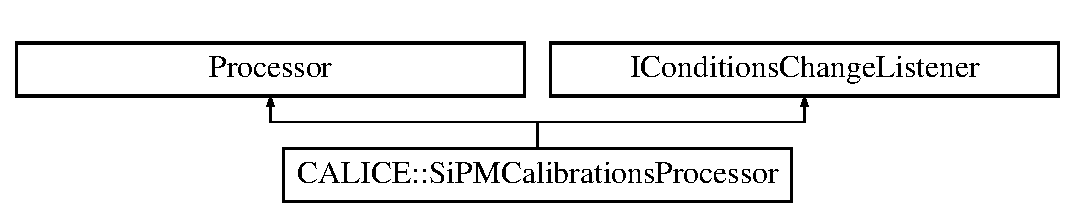
\includegraphics[height=2.000000cm]{classCALICE_1_1SiPMCalibrationsProcessor}
\end{center}
\end{figure}
\subsection*{Public Member Functions}
\begin{DoxyCompactItemize}
\item 
virtual Processor $\ast$ {\bfseries new\-Processor} ()\label{classCALICE_1_1SiPMCalibrationsProcessor_a09bc600c6c5e0aee2d44c30ffcdf27c1}

\item 
virtual void {\bfseries init} ()\label{classCALICE_1_1SiPMCalibrationsProcessor_a0d9c1955bda51b03f0a8717f4380b7e0}

\item 
virtual void {\bfseries process\-Event} (L\-C\-Event $\ast$evt)\label{classCALICE_1_1SiPMCalibrationsProcessor_a4a9b57072973e4de373a83d01292cbd1}

\item 
virtual void {\bfseries end} ()\label{classCALICE_1_1SiPMCalibrationsProcessor_ada3d8906c4cb52b6154b9aef7f3ea491}

\item 
virtual void {\bfseries conditions\-Changed} (L\-C\-Collection $\ast$col)\label{classCALICE_1_1SiPMCalibrationsProcessor_a6d5ea5244129f8f36bce7491f88475e2}

\end{DoxyCompactItemize}
\subsection*{Static Public Member Functions}
\begin{DoxyCompactItemize}
\item 
static Mapped\-Container\\*
$<$ Si\-P\-M\-Calibrations $>$ $\ast$ {\bf get\-Calibrations} (const std\-::string \&processor\-Name)
\begin{DoxyCompactList}\small\item\em static function to obtain a Mapped\-Container with cell neighbours \end{DoxyCompactList}\end{DoxyCompactItemize}
\subsection*{Private Member Functions}
\begin{DoxyCompactItemize}
\item 
void {\bfseries update\-Mapping} ()\label{classCALICE_1_1SiPMCalibrationsProcessor_a9e3ec26b7c119de987cb7e3061963b44}

\item 
void {\bfseries update\-M\-I\-P\-Calibration} ()\label{classCALICE_1_1SiPMCalibrationsProcessor_ace11b437347007d6490bbdba8250c256}

\item 
void {\bfseries update\-Gain\-Calibration} ()\label{classCALICE_1_1SiPMCalibrationsProcessor_a43dd0463641ba8b751bab0681dd3111b}

\item 
void {\bfseries update\-Pedestal} ()\label{classCALICE_1_1SiPMCalibrationsProcessor_a3ba7c1647f7b070b57f96c2106234ddc}

\item 
void {\bfseries update\-Temperature} ()\label{classCALICE_1_1SiPMCalibrationsProcessor_adb1538dd10bdc151279a0d3e957deabd}

\item 
void {\bfseries update\-Inter\-Calibration} ()\label{classCALICE_1_1SiPMCalibrationsProcessor_a4d50b20e4472ae066e4f3c1c9eaae1be}

\item 
void {\bfseries update\-Saturation} ()\label{classCALICE_1_1SiPMCalibrationsProcessor_a433a2317a197497d9afab19754a107a8}

\item 
void {\bfseries update\-Cell\-Quality} ()\label{classCALICE_1_1SiPMCalibrationsProcessor_a04ce651a0aae014bbd381b1d71031e64}

\end{DoxyCompactItemize}
\subsection*{Private Attributes}
\begin{DoxyCompactItemize}
\item 
Mapped\-Container\\*
$<$ Si\-P\-M\-Calibrations $>$ $\ast$ {\bfseries \-\_\-container}\label{classCALICE_1_1SiPMCalibrationsProcessor_a96e31d9477a05cccc60f529680f3344d}

\item 
std\-::vector$<$ Si\-P\-M\-Calibrations $\ast$ $>$ {\bfseries \-\_\-all\-Calibrations}\label{classCALICE_1_1SiPMCalibrationsProcessor_a6f20a968a0f4693f704e699809315b5c}

\item 
std\-::string {\bfseries \-\_\-mapping\-Processor\-Name}\label{classCALICE_1_1SiPMCalibrationsProcessor_ac22335161395b377e2af826a5c67f327}

\item 
std\-::string {\bfseries \-\_\-\-M\-I\-P\-Constant\-Col\-Name}\label{classCALICE_1_1SiPMCalibrationsProcessor_a4d165809c34d6a8a9260a3d0852a3e20}

\item 
std\-::string {\bfseries \-\_\-\-M\-I\-P\-Slope\-Col\-Name}\label{classCALICE_1_1SiPMCalibrationsProcessor_a7ecd098aa4c32f9c87e5b2576e886e1c}

\item 
std\-::string {\bfseries \-\_\-gain\-Constant\-Col\-Name}\label{classCALICE_1_1SiPMCalibrationsProcessor_a416de670db12ec96a47228d5a860a69c}

\item 
std\-::string {\bfseries \-\_\-gain\-Slope\-Col\-Name}\label{classCALICE_1_1SiPMCalibrationsProcessor_aef0180e8fcb6850e6aba5c755b8ad145}

\item 
std\-::string {\bfseries \-\_\-inter\-Calibration\-Col\-Name}\label{classCALICE_1_1SiPMCalibrationsProcessor_a4a7a7946644e333764897e9d33110cdb}

\item 
std\-::string {\bfseries \-\_\-pedestal\-Col\-Name}\label{classCALICE_1_1SiPMCalibrationsProcessor_a1fdf8e0463512673609a6469fe12312b}

\item 
std\-::string {\bfseries \-\_\-temperature\-Col\-Name}\label{classCALICE_1_1SiPMCalibrationsProcessor_ae43734518172f8ddac288ca9a62af99c}

\item 
std\-::string {\bfseries \-\_\-saturation\-Col\-Name}\label{classCALICE_1_1SiPMCalibrationsProcessor_ab81f969e03c7a7011672e0f33f0f8838}

\item 
std\-::string {\bfseries \-\_\-saturation\-Parameters\-Col\-Name}\label{classCALICE_1_1SiPMCalibrationsProcessor_a3b31c71ec1a92a720716c3fe4a425016}

\item 
std\-::string {\bfseries \-\_\-pixel\-Scale\-Factors\-Col\-Name}\label{classCALICE_1_1SiPMCalibrationsProcessor_accb68a3b84fc5197a1350c038b08c841}

\item 
std\-::string {\bfseries \-\_\-cell\-Quality\-Col\-Name}\label{classCALICE_1_1SiPMCalibrationsProcessor_a9d560eeee8dafe396777c1c6a5d58834}

\item 
L\-C\-Collection $\ast$ {\bfseries \-\_\-\-M\-I\-P\-Constant\-Col}\label{classCALICE_1_1SiPMCalibrationsProcessor_a7da743bf97f6b3e94f0a1a5df6703e6a}

\item 
L\-C\-Collection $\ast$ {\bfseries \-\_\-\-M\-I\-P\-Slope\-Col}\label{classCALICE_1_1SiPMCalibrationsProcessor_ae6ae8c0999422d805f87e5aece93f4ce}

\item 
L\-C\-Collection $\ast$ {\bfseries \-\_\-gain\-Constant\-Col}\label{classCALICE_1_1SiPMCalibrationsProcessor_a06ce1acf741b1126d1e6260961469310}

\item 
L\-C\-Collection $\ast$ {\bfseries \-\_\-gain\-Slope\-Col}\label{classCALICE_1_1SiPMCalibrationsProcessor_a1b81d42f8d3bc674e4b90157226ae3a3}

\item 
L\-C\-Collection $\ast$ {\bfseries \-\_\-inter\-Calibration\-Col}\label{classCALICE_1_1SiPMCalibrationsProcessor_a0573c61704727ceccdbe88cdf18d74d2}

\item 
L\-C\-Collection $\ast$ {\bfseries \-\_\-pedestal\-Col}\label{classCALICE_1_1SiPMCalibrationsProcessor_a3e949491283ca2fddad6b5cb9210aba7}

\item 
L\-C\-Collection $\ast$ {\bfseries \-\_\-temperature\-Col}\label{classCALICE_1_1SiPMCalibrationsProcessor_a7ddbaec5d8e540df22346e180ef570e0}

\item 
L\-C\-Collection $\ast$ {\bfseries \-\_\-saturation\-Col}\label{classCALICE_1_1SiPMCalibrationsProcessor_a2bbe3bb6d0d94bd95c209a65f018d189}

\item 
L\-C\-Collection $\ast$ {\bfseries \-\_\-saturation\-Parameters\-Col}\label{classCALICE_1_1SiPMCalibrationsProcessor_af87a35b0bb7c078466d6e7beb7046463}

\item 
L\-C\-Collection $\ast$ {\bfseries \-\_\-pixel\-Scale\-Factors\-Col}\label{classCALICE_1_1SiPMCalibrationsProcessor_ac807c9abda924e2e7575b1bf6359b5f3}

\item 
L\-C\-Collection $\ast$ {\bfseries \-\_\-cell\-Quality\-Col}\label{classCALICE_1_1SiPMCalibrationsProcessor_a89d41d718d254530864d0ddf2b234849}

\item 
bool {\bfseries \-\_\-\-M\-I\-P\-Constant\-Changed}\label{classCALICE_1_1SiPMCalibrationsProcessor_aa788a1748b9d268fb0361a8617562de4}

\item 
bool {\bfseries \-\_\-\-M\-I\-P\-Slope\-Changed}\label{classCALICE_1_1SiPMCalibrationsProcessor_a4879ecb81772ff533ad5dfa9b39c467c}

\item 
bool {\bfseries \-\_\-gain\-Constant\-Changed}\label{classCALICE_1_1SiPMCalibrationsProcessor_abd8f8baf7dc83fda0896932ec1148509}

\item 
bool {\bfseries \-\_\-gain\-Slope\-Changed}\label{classCALICE_1_1SiPMCalibrationsProcessor_a7695599d5a146b69e9793e105b10a65a}

\item 
bool {\bfseries \-\_\-inter\-Calibration\-Changed}\label{classCALICE_1_1SiPMCalibrationsProcessor_ac449330e6eab8344207af2be0f8b63ae}

\item 
bool {\bfseries \-\_\-pedestal\-Changed}\label{classCALICE_1_1SiPMCalibrationsProcessor_a29f4c7d6e864ec715a34965ed1861a54}

\item 
bool {\bfseries \-\_\-temperature\-Changed}\label{classCALICE_1_1SiPMCalibrationsProcessor_a2626e03c9ac090a21b5f7e24f5d3fb51}

\item 
bool {\bfseries \-\_\-saturation\-Changed}\label{classCALICE_1_1SiPMCalibrationsProcessor_a985defc7240eb6e5aa4455c4c2386108}

\item 
bool {\bfseries \-\_\-saturation\-Parameters\-Changed}\label{classCALICE_1_1SiPMCalibrationsProcessor_a38855b53523989e9eccdcb36d14dac35}

\item 
bool {\bfseries \-\_\-pixel\-Scale\-Factors\-Changed}\label{classCALICE_1_1SiPMCalibrationsProcessor_a96bcc0952d1aa9dc9077d8b3d988032b}

\item 
bool {\bfseries \-\_\-cell\-Quality\-Changed}\label{classCALICE_1_1SiPMCalibrationsProcessor_abc67109ca636df5bd458a99524cc0712}

\item 
bool {\bfseries \-\_\-use\-D\-B\-Default\-Values\-Only}\label{classCALICE_1_1SiPMCalibrationsProcessor_aad04fab65320e8d1495d42b106b5592e}

\item 
bool {\bfseries \-\_\-use\-Individual\-Scale\-Factor}\label{classCALICE_1_1SiPMCalibrationsProcessor_ac8ab414d62ad74b0e2bdf9642a57d0cc}

\item 
float {\bfseries \-\_\-global\-Pixel\-Scale\-Factor}\label{classCALICE_1_1SiPMCalibrationsProcessor_a09aa18a64fcf99504bac4e3bfd354f95}

\item 
int {\bfseries \-\_\-saturation\-Procedure\-Type}\label{classCALICE_1_1SiPMCalibrationsProcessor_a665116398e2a62bd0db4f5b6d9cfa8c1}

\item 
bool {\bfseries \-\_\-\-M\-I\-P\-Constant\-Scaled}\label{classCALICE_1_1SiPMCalibrationsProcessor_a78714e85fbfdfd8da3106b82503ae45f}

\item 
bool {\bfseries \-\_\-\-M\-I\-P\-Slope\-Scaled}\label{classCALICE_1_1SiPMCalibrationsProcessor_ab30bd5f16cddec106bdbe9205fc0e988}

\item 
bool {\bfseries \-\_\-gain\-Constant\-Scaled}\label{classCALICE_1_1SiPMCalibrationsProcessor_ac5ff69945eb2c6d371f474e72ecd06c8}

\item 
bool {\bfseries \-\_\-gain\-Slope\-Scaled}\label{classCALICE_1_1SiPMCalibrationsProcessor_a4cedf6248e8323b30d1a049a4b7842e9}

\item 
bool {\bfseries \-\_\-inter\-Calibration\-Scaled}\label{classCALICE_1_1SiPMCalibrationsProcessor_a984cf4c886be6b7569ad0544178b2443}

\item 
bool {\bfseries \-\_\-saturation\-Correction\-Scaled}\label{classCALICE_1_1SiPMCalibrationsProcessor_a50086a8098d775c7271db770eb4b2951}

\item 
float {\bfseries \-\_\-\-M\-I\-P\-Constant\-Scale\-Factor}\label{classCALICE_1_1SiPMCalibrationsProcessor_ade64d1fed1edc3cd13a23a399908da4c}

\item 
float {\bfseries \-\_\-\-M\-I\-P\-Slope\-Scale\-Factor}\label{classCALICE_1_1SiPMCalibrationsProcessor_afbca1f8f9b81c4dd99c68b8c278faba8}

\item 
float {\bfseries \-\_\-gain\-Constant\-Scale\-Factor}\label{classCALICE_1_1SiPMCalibrationsProcessor_a9bd9189079825224dbeff4c7dc41f1f9}

\item 
float {\bfseries \-\_\-gain\-Slope\-Scale\-Factor}\label{classCALICE_1_1SiPMCalibrationsProcessor_a3084193d9d41e8a1a486c08a8e865bfc}

\item 
float {\bfseries \-\_\-inter\-Calibration\-Scale\-Factor}\label{classCALICE_1_1SiPMCalibrationsProcessor_af50ac678d86d3a392dd1d86a3a6b8433}

\item 
float {\bfseries \-\_\-saturation\-Correction\-Scale\-Factor}\label{classCALICE_1_1SiPMCalibrationsProcessor_ac0156a87686b55f990953686d540ae70}

\item 
const Mapper $\ast$ {\bfseries \-\_\-mapper}\label{classCALICE_1_1SiPMCalibrationsProcessor_a1520ccc4bc259fd6913c134259072fd7}

\item 
unsigned int {\bfseries \-\_\-mapper\-Version}\label{classCALICE_1_1SiPMCalibrationsProcessor_a3d89c10e7c8dd2481dd32f01771508d3}

\end{DoxyCompactItemize}
\subsection*{Static Private Attributes}
\begin{DoxyCompactItemize}
\item 
static std\-::map$<$ std\-::string, \\*
Mapped\-Container\\*
$<$ Si\-P\-M\-Calibrations $>$ $\ast$ $>$ {\bfseries \-\_\-\-Si\-P\-M\-Calibrations\-Container\-Map}\label{classCALICE_1_1SiPMCalibrationsProcessor_a4bc42b8329f9f12e0168ff50b4f1cfcc}

\end{DoxyCompactItemize}


\subsection{Detailed Description}
Processor that provides Si\-P\-M calibration information to other processors. 

To obtain the object in other processors use\-: \doxyref{Si\-P\-M\-Calibrations\-Processor\-::get\-Calibrations}{p.}{classCALICE_1_1SiPMCalibrationsProcessor_a3e2a886b4bb05522e0f8313aed6238b7}( \char`\"{}\-Si\-P\-M\-Calibrations processor name\char`\"{} )

\begin{DoxyParagraph}{processor parameters}
\begin{TabularC}{2}
\hline
steering file parameter name &description  \\\cline{1-2}
{\bfseries {\itshape  Mapping\-Processor\-Name }}&name of the mapping processor that provides the necessary Mapper class \\\cline{1-2}
{\bfseries {\itshape  Mip\-Constant\-Collection }}&name of the M\-I\-P constants collection \\\cline{1-2}
{\bfseries {\itshape  Mip\-Slopes\-Collection }}&name of the M\-I\-P slopes collection \\\cline{1-2}
{\bfseries {\itshape  Gain\-Constant\-Collection }}&name of the gain constants collection \\\cline{1-2}
{\bfseries {\itshape  Gain\-Slope\-Collection }}&name of the gain slopes collection \\\cline{1-2}
{\bfseries {\itshape  Pedestal\-Collection }}&name of the pedestal collection \\\cline{1-2}
{\bfseries {\itshape  Saturation\-Collection }}&name of the saturation collection \\\cline{1-2}
{\bfseries {\itshape  Pixel\-Scale\-Factors\-Collection }}&name of the pixel scale factors collection \\\cline{1-2}
{\bfseries {\itshape  Global\-Pixel\-Scale\-Factor }}&global value for the pixel scale factor \\\cline{1-2}
{\bfseries {\itshape  Cell\-Quality\-Collection }}&name of the saturation collection \\\cline{1-2}
\end{TabularC}

\end{DoxyParagraph}
\begin{DoxyAuthor}{Author}
{\tt Benjamin.\-Lutz@desy.\-de} 
\end{DoxyAuthor}
\begin{DoxyVersion}{Version}
0.\-1 
\end{DoxyVersion}
\begin{DoxyDate}{Date}
October 2009 
\end{DoxyDate}


Definition at line 58 of file Si\-P\-M\-Calibrations\-Processor.\-hh.



\subsection{Member Function Documentation}
\index{C\-A\-L\-I\-C\-E\-::\-Si\-P\-M\-Calibrations\-Processor@{C\-A\-L\-I\-C\-E\-::\-Si\-P\-M\-Calibrations\-Processor}!get\-Calibrations@{get\-Calibrations}}
\index{get\-Calibrations@{get\-Calibrations}!CALICE::SiPMCalibrationsProcessor@{C\-A\-L\-I\-C\-E\-::\-Si\-P\-M\-Calibrations\-Processor}}
\subsubsection[{get\-Calibrations}]{\setlength{\rightskip}{0pt plus 5cm}Mapped\-Container$<$ Si\-P\-M\-Calibrations $>$ $\ast$ C\-A\-L\-I\-C\-E\-::\-Si\-P\-M\-Calibrations\-Processor\-::get\-Calibrations (
\begin{DoxyParamCaption}
\item[{const std\-::string \&}]{processor\-Name}
\end{DoxyParamCaption}
)\hspace{0.3cm}{\ttfamily [static]}}\label{classCALICE_1_1SiPMCalibrationsProcessor_a3e2a886b4bb05522e0f8313aed6238b7}


static function to obtain a Mapped\-Container with cell neighbours 


\begin{DoxyParams}[1]{Parameters}
\mbox{\tt in}  & {\em processor\-Name} & name of the \doxyref{Si\-P\-M\-Calibrations\-Processor}{p.}{classCALICE_1_1SiPMCalibrationsProcessor} that takes care of this Si\-P\-M\-Calibrations. \\
\hline
\end{DoxyParams}
\begin{DoxyReturn}{Returns}
pointer to the Mapped\-Container including Si\-P\-M\-Calibrations 
\end{DoxyReturn}


Definition at line 32 of file Si\-P\-M\-Calibrations\-Processor.\-cc.



Referenced by C\-A\-L\-I\-C\-E\-::\-Si\-P\-M\-Calibrate\-Processor\-::init().



The documentation for this class was generated from the following files\-:\begin{DoxyCompactItemize}
\item 
Si\-P\-M\-Calibrations\-Processor.\-hh\item 
Si\-P\-M\-Calibrations\-Processor.\-cc\end{DoxyCompactItemize}

\section{C\-A\-L\-I\-C\-E\-:\-:Si\-P\-M\-Temperature\-Processor Class Reference}
\label{classCALICE_1_1SiPMTemperatureProcessor}\index{C\-A\-L\-I\-C\-E\-::\-Si\-P\-M\-Temperature\-Processor@{C\-A\-L\-I\-C\-E\-::\-Si\-P\-M\-Temperature\-Processor}}


Processor that provides the Si\-P\-M temperature.  




{\ttfamily \#include $<$Si\-P\-M\-Temperature\-Processor.\-hh$>$}

Inheritance diagram for C\-A\-L\-I\-C\-E\-:\-:Si\-P\-M\-Temperature\-Processor\-:\begin{figure}[H]
\begin{center}
\leavevmode
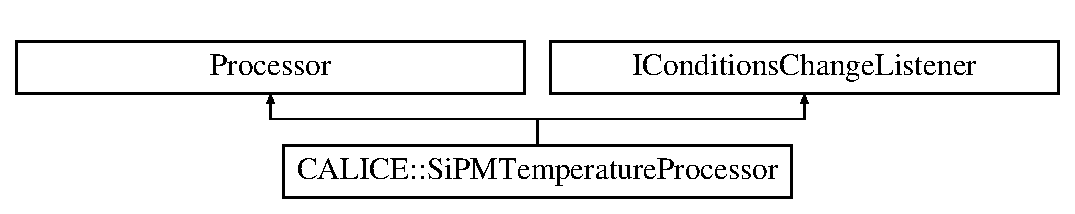
\includegraphics[height=2.000000cm]{classCALICE_1_1SiPMTemperatureProcessor}
\end{center}
\end{figure}
\subsection*{Public Member Functions}
\begin{DoxyCompactItemize}
\item 
{\bf Si\-P\-M\-Temperature\-Processor} ()\label{classCALICE_1_1SiPMTemperatureProcessor_a04ac0bf7f828c454fb8dada5710e5106}

\begin{DoxyCompactList}\small\item\em Default constructor. \end{DoxyCompactList}\item 
{\bf $\sim$\-Si\-P\-M\-Temperature\-Processor} ()\label{classCALICE_1_1SiPMTemperatureProcessor_ac484602a86c82558880b3ebc1f62dc77}

\begin{DoxyCompactList}\small\item\em Destructor. \end{DoxyCompactList}\item 
virtual {\bf Si\-P\-M\-Temperature\-Processor} $\ast$ {\bf new\-Processor} ()\label{classCALICE_1_1SiPMTemperatureProcessor_ad65bd44b3ce6be3260e57c1fcb75dcba}

\begin{DoxyCompactList}\small\item\em Return a new instance of the processor. \end{DoxyCompactList}\item 
virtual void {\bf init} ()\label{classCALICE_1_1SiPMTemperatureProcessor_a900fb4beaa66160686582a75c7fe2968}

\begin{DoxyCompactList}\small\item\em Called at the begin of the job before anything is read. \end{DoxyCompactList}\item 
virtual void {\bf process\-Event} (L\-C\-Event $\ast$evt)
\begin{DoxyCompactList}\small\item\em Called for every event. \end{DoxyCompactList}\item 
virtual void {\bf end} ()\label{classCALICE_1_1SiPMTemperatureProcessor_a2cbda0153aeecea1be18a5a1b9eadb65}

\begin{DoxyCompactList}\small\item\em Called after data processing (after all events are processed) for clean up. \end{DoxyCompactList}\item 
virtual void {\bf conditions\-Changed} (L\-C\-Collection $\ast$col)
\begin{DoxyCompactList}\small\item\em Callback function for the condition changes. \end{DoxyCompactList}\end{DoxyCompactItemize}
\subsection*{Static Public Member Functions}
\begin{DoxyCompactItemize}
\item 
static Ahc\-Temp\-Provider $\ast$ {\bf get\-Temperature\-Provider} (const std\-::string \&processor\-Name)
\begin{DoxyCompactList}\small\item\em Get the temperature provider. \end{DoxyCompactList}\end{DoxyCompactItemize}
\subsection*{Private Attributes}
\begin{DoxyCompactItemize}
\item 
std\-::string {\bf \-\_\-ahc\-Sro\-Mod\-Data\-Col\-Name}\label{classCALICE_1_1SiPMTemperatureProcessor_a20b373be23412e6f4c10fb83f341c365}

\begin{DoxyCompactList}\small\item\em name of the collection containing the slow control data \end{DoxyCompactList}\item 
std\-::string {\bf \-\_\-temperature\-Sensor\-Calibration\-Col\-Name}\label{classCALICE_1_1SiPMTemperatureProcessor_a7f729d260699eb7bac4949150379b621}

\begin{DoxyCompactList}\small\item\em name of the collection containing the temperature sensor calibration \end{DoxyCompactList}\item 
L\-C\-Collection $\ast$ {\bf \-\_\-ahc\-Sro\-Mod\-Data\-Col}\label{classCALICE_1_1SiPMTemperatureProcessor_ab6f1a7bd77b6d74ad05d28ae00f92a96}

\begin{DoxyCompactList}\small\item\em collection containing the slow control data \end{DoxyCompactList}\item 
L\-C\-Collection $\ast$ {\bf \-\_\-temperature\-Sensor\-Calibration\-Col}\label{classCALICE_1_1SiPMTemperatureProcessor_a83f01ec9192ad50fa91b8ef05bbfe0d1}

\begin{DoxyCompactList}\small\item\em collection containing the temperature sensor calibration \end{DoxyCompactList}\item 
bool {\bf \-\_\-ahc\-Sro\-Mod\-Data\-Col\-Changed}\label{classCALICE_1_1SiPMTemperatureProcessor_addb8e35a9df5dea954ea49672e467fe3}

\begin{DoxyCompactList}\small\item\em flag to signalise if the slow control data collection has changed \end{DoxyCompactList}\item 
bool {\bf \-\_\-temperature\-Sensor\-Calibration\-Col\-Changed}\label{classCALICE_1_1SiPMTemperatureProcessor_af6e3e77f027c314019afaa41617dc57f}

\begin{DoxyCompactList}\small\item\em flag to signalise if the collection containing the temperature sensor calibration hass changed or not \end{DoxyCompactList}\item 
std\-::string {\bf \-\_\-mapping\-Processor\-Name}\label{classCALICE_1_1SiPMTemperatureProcessor_a1068bf0ac9a36c77aeefaf03514bd5e8}

\begin{DoxyCompactList}\small\item\em name of the processor name which provides the mapping \end{DoxyCompactList}\item 
Ahc\-Temp\-Provider $\ast$ {\bf \-\_\-temp\-Provider}\label{classCALICE_1_1SiPMTemperatureProcessor_ab874014a3ab396472b48b7533c9316b5}

\begin{DoxyCompactList}\small\item\em pointer to the A\-H\-C temperature provider \end{DoxyCompactList}\item 
const Ahc\-Mapper $\ast$ {\bf \-\_\-mapper}\label{classCALICE_1_1SiPMTemperatureProcessor_addf40c4cb0947b2bb138012bfcf31de6}

\begin{DoxyCompactList}\small\item\em the mapper \end{DoxyCompactList}\item 
lcio\-::\-Float\-Vec {\bf \-\_\-temp\-Provider\-Sanity\-Range\-Vec}\label{classCALICE_1_1SiPMTemperatureProcessor_a0bb6fba3c3e3cab14180259a473fe526}

\begin{DoxyCompactList}\small\item\em vector of floats to save the sanity range of the temperature provider \end{DoxyCompactList}\item 
std\-::string {\bf \-\_\-temp\-Provider\-Model\-Name}
\begin{DoxyCompactList}\small\item\em name of the model used for the temperature provider. \end{DoxyCompactList}\item 
std\-::string {\bf \-\_\-output\-Col\-Name}\label{classCALICE_1_1SiPMTemperatureProcessor_a583ed1ec93ef7e553c95ea291b51cb55}

\begin{DoxyCompactList}\small\item\em name of the output collection \end{DoxyCompactList}\item 
L\-C\-Collection $\ast$ {\bf \-\_\-col\-Temperature}\label{classCALICE_1_1SiPMTemperatureProcessor_adbf2244effa4e4902692663a4c0f71a8}

\begin{DoxyCompactList}\small\item\em collection of temperatures \end{DoxyCompactList}\item 
Run\-Time\-Conditions\-Handler $\ast$ {\bf \-\_\-conditions\-Handler}\label{classCALICE_1_1SiPMTemperatureProcessor_a40bb02477d3ab8f01a0d5ca7ee1040a8}

\begin{DoxyCompactList}\small\item\em pointer to the run time conditions handler \end{DoxyCompactList}\end{DoxyCompactItemize}
\subsection*{Static Private Attributes}
\begin{DoxyCompactItemize}
\item 
static std\-::map$<$ std\-::string, \\*
Ahc\-Temp\-Provider $\ast$ $>$ {\bf \-\_\-temp\-Provider\-Map}\label{classCALICE_1_1SiPMTemperatureProcessor_ae29d242598f44f0dc52051a3119fbdbe}

\begin{DoxyCompactList}\small\item\em map of Ahc\-Temp\-Provider \end{DoxyCompactList}\end{DoxyCompactItemize}


\subsection{Detailed Description}
Processor that provides the Si\-P\-M temperature. 

The processor generates and updates a C\-A\-L\-I\-C\-E Mapped\-Container object from the conditions data. To obtain the object in other processors use\-: Si\-P\-M\-Temperature\-Processor\-::get\-Temperature\-Container(\char`\"{}temperature processor name\char`\"{});

\begin{DoxyAuthor}{Author}
{\tt angela-\/isabela.\-lucaci-\/timoce@desy.\-de} 
\end{DoxyAuthor}
\begin{DoxyVersion}{Version}
0.\-2 
\end{DoxyVersion}
\begin{DoxyDate}{Date}
May 2010 
\end{DoxyDate}


Definition at line 36 of file Si\-P\-M\-Temperature\-Processor.\-hh.



\subsection{Member Function Documentation}
\index{C\-A\-L\-I\-C\-E\-::\-Si\-P\-M\-Temperature\-Processor@{C\-A\-L\-I\-C\-E\-::\-Si\-P\-M\-Temperature\-Processor}!conditions\-Changed@{conditions\-Changed}}
\index{conditions\-Changed@{conditions\-Changed}!CALICE::SiPMTemperatureProcessor@{C\-A\-L\-I\-C\-E\-::\-Si\-P\-M\-Temperature\-Processor}}
\subsubsection[{conditions\-Changed}]{\setlength{\rightskip}{0pt plus 5cm}void C\-A\-L\-I\-C\-E\-::\-Si\-P\-M\-Temperature\-Processor\-::conditions\-Changed (
\begin{DoxyParamCaption}
\item[{L\-C\-Collection $\ast$}]{col}
\end{DoxyParamCaption}
)\hspace{0.3cm}{\ttfamily [virtual]}}\label{classCALICE_1_1SiPMTemperatureProcessor_a05aa832ece6bc5253418e56db9e79cf7}


Callback function for the condition changes. 


\begin{DoxyParams}{Parameters}
{\em col} & collection to be checked if it has changed or not \\
\hline
\end{DoxyParams}


Definition at line 168 of file Si\-P\-M\-Temperature\-Processor.\-cc.



References \-\_\-ahc\-Sro\-Mod\-Data\-Col, \-\_\-ahc\-Sro\-Mod\-Data\-Col\-Changed, \-\_\-ahc\-Sro\-Mod\-Data\-Col\-Name, \-\_\-temperature\-Sensor\-Calibration\-Col, \-\_\-temperature\-Sensor\-Calibration\-Col\-Changed, and \-\_\-temperature\-Sensor\-Calibration\-Col\-Name.

\index{C\-A\-L\-I\-C\-E\-::\-Si\-P\-M\-Temperature\-Processor@{C\-A\-L\-I\-C\-E\-::\-Si\-P\-M\-Temperature\-Processor}!get\-Temperature\-Provider@{get\-Temperature\-Provider}}
\index{get\-Temperature\-Provider@{get\-Temperature\-Provider}!CALICE::SiPMTemperatureProcessor@{C\-A\-L\-I\-C\-E\-::\-Si\-P\-M\-Temperature\-Processor}}
\subsubsection[{get\-Temperature\-Provider}]{\setlength{\rightskip}{0pt plus 5cm}Ahc\-Temp\-Provider $\ast$ C\-A\-L\-I\-C\-E\-::\-Si\-P\-M\-Temperature\-Processor\-::get\-Temperature\-Provider (
\begin{DoxyParamCaption}
\item[{const std\-::string \&}]{processor\-Name}
\end{DoxyParamCaption}
)\hspace{0.3cm}{\ttfamily [static]}}\label{classCALICE_1_1SiPMTemperatureProcessor_ae53699ce851320ce9b964a49f54da2c9}


Get the temperature provider. 


\begin{DoxyParams}{Parameters}
{\em processor\-Name} & name of the processor returning the temperature provider \\
\hline
\end{DoxyParams}
\begin{DoxyReturn}{Returns}
Ahc\-Temp\-Provider 
\end{DoxyReturn}


Definition at line 34 of file Si\-P\-M\-Temperature\-Processor.\-cc.



References \-\_\-temp\-Provider\-Map.

\index{C\-A\-L\-I\-C\-E\-::\-Si\-P\-M\-Temperature\-Processor@{C\-A\-L\-I\-C\-E\-::\-Si\-P\-M\-Temperature\-Processor}!process\-Event@{process\-Event}}
\index{process\-Event@{process\-Event}!CALICE::SiPMTemperatureProcessor@{C\-A\-L\-I\-C\-E\-::\-Si\-P\-M\-Temperature\-Processor}}
\subsubsection[{process\-Event}]{\setlength{\rightskip}{0pt plus 5cm}void C\-A\-L\-I\-C\-E\-::\-Si\-P\-M\-Temperature\-Processor\-::process\-Event (
\begin{DoxyParamCaption}
\item[{L\-C\-Event $\ast$}]{evt}
\end{DoxyParamCaption}
)\hspace{0.3cm}{\ttfamily [virtual]}}\label{classCALICE_1_1SiPMTemperatureProcessor_a9724f37f98d88c56707192b3ccd8f778}


Called for every event. 


\begin{DoxyParams}{Parameters}
{\em evt} & event to be processed \\
\hline
\end{DoxyParams}


Definition at line 196 of file Si\-P\-M\-Temperature\-Processor.\-cc.



References \-\_\-ahc\-Sro\-Mod\-Data\-Col, \-\_\-ahc\-Sro\-Mod\-Data\-Col\-Changed, \-\_\-ahc\-Sro\-Mod\-Data\-Col\-Name, \-\_\-col\-Temperature, \-\_\-conditions\-Handler, \-\_\-mapper, \-\_\-temperature\-Sensor\-Calibration\-Col, \-\_\-temperature\-Sensor\-Calibration\-Col\-Changed, \-\_\-temperature\-Sensor\-Calibration\-Col\-Name, and \-\_\-temp\-Provider.



\subsection{Field Documentation}
\index{C\-A\-L\-I\-C\-E\-::\-Si\-P\-M\-Temperature\-Processor@{C\-A\-L\-I\-C\-E\-::\-Si\-P\-M\-Temperature\-Processor}!\-\_\-temp\-Provider\-Model\-Name@{\-\_\-temp\-Provider\-Model\-Name}}
\index{\-\_\-temp\-Provider\-Model\-Name@{\-\_\-temp\-Provider\-Model\-Name}!CALICE::SiPMTemperatureProcessor@{C\-A\-L\-I\-C\-E\-::\-Si\-P\-M\-Temperature\-Processor}}
\subsubsection[{\-\_\-temp\-Provider\-Model\-Name}]{\setlength{\rightskip}{0pt plus 5cm}std\-::string C\-A\-L\-I\-C\-E\-::\-Si\-P\-M\-Temperature\-Processor\-::\-\_\-temp\-Provider\-Model\-Name\hspace{0.3cm}{\ttfamily [private]}}\label{classCALICE_1_1SiPMTemperatureProcessor_afdc26a29605485025b7f81dbc3c24aee}


name of the model used for the temperature provider. 

If the model is \char`\"{}simple\char`\"{}, use Ahc\-Simple\-Temp\-Provider 

Definition at line 101 of file Si\-P\-M\-Temperature\-Processor.\-hh.



Referenced by init(), and Si\-P\-M\-Temperature\-Processor().



The documentation for this class was generated from the following files\-:\begin{DoxyCompactItemize}
\item 
Si\-P\-M\-Temperature\-Processor.\-hh\item 
Si\-P\-M\-Temperature\-Processor.\-cc\end{DoxyCompactItemize}

%--- End generated contents ---

% Index
\newpage
\phantomsection
\addcontentsline{toc}{part}{Index}
\printindex

\end{document}
